\documentclass[a4paper]{jsbook}
%\documentclass[a4paper,oneside]{jsbook} % 片面刷りの場合は oneside を追加
%\documentclass[a4paper,openany]{jsbook} % 章末の白紙ページを省きたいとき

\usepackage[sort]{cite}              % 参考文献のソート
\usepackage[dvipdfmx]{color}
\usepackage{listings}
\usepackage{comment}
\usepackage{ascmac}

%%% for make figures in one page
\renewcommand\floatpagefraction{.001}
\makeatletter
\setlength\@fpsep{\textheight}
\makeatother
%%%

\mathchardef\mhyphen="2D
\def\ra{\rightarrow}
\def\Ra{\Rightarrow}
\newcommand{\minconf}{mincon\!f}
\newcommand{\confidence}{con\!f\!idence}
\newcommand{\fmeasure}{F\mhyphen measure}



\renewcommand{\lstlistingname}{リスト}

\definecolor{gray}{rgb}{0.4,0.4,0.4}
\definecolor{darkblue}{rgb}{0.0,0.0,0.6}
\definecolor{cyan}{rgb}{0.0,0.6,0.6}

\lstset{
  basicstyle={\scriptsize\ttfamily},
  columns=fullflexible,
  showstringspaces=false,
  commentstyle=\color{gray}\upshape,
  breaklines=true
}
\lstdefinestyle{normalsize}{
  basicstyle={\ttfamily}
}

\lstdefinelanguage{XML}
{
  morestring=[b]",
  morestring=[s]{>}{<},
  morecomment=[s]{<?}{?>},
  stringstyle=\color{black},
  identifierstyle=\color{darkblue},
  keywordstyle=\color{cyan},
  morekeywords={xmlns,version,type}% list your attributes here
}


\usepackage[mthesis,draft]{salab}    % 草稿では draft を追加
%\usepackage[mthesis]{salab}         % 本番はこっち




\hyphenpenalty=10000

\title{細粒度操作履歴の分析に基づく\\開発行動推薦}
\author{山森 章弘}
\authorintitle{山~~森~~~~~章~~弘} % 表示用
\date{平成28年1月}
\nendo{平成27}
\studentid{14M38439}
\advisor{小林 隆志 准教授}
\affiliation{大学院情報理工学研究科 計算工学専攻}

\begin{document}

\frontmatter
\maketitle

\chapter*{概要}
本論文では,...
\TODO{}

\chapter*{Abstract}
This dissertation studies ...
\TODO{}

\tableofcontents
\listoffigures
\listoftables

\mainmatter
% 章番号が決まったらファイル名に連番を振っても良いし,
% include せずにすべてをこのファイルに含めても良い.

\chapter{序論}
\section{背景}
ソフトウェアの大規模化に伴い、メンテナンス時のバグ修正や機能追加タスクの作業で必要な依存関係解決の作業量は増大している。
ソフトウェアの品質を向上させるため、メンテナンス作業中に変更の必要なソースコードを全て列挙できることは重要であり、この作業を支援する研究は変更支援(change guide)と呼ばれている。
変更支援のうち、静的解析に基づき、ソースコードの依存関係をもとに変更伝搬箇所を特定する手法が提案されている\cite{792645}が、
この手法は膨大な量の依存関係を解析するため計算量が多く、また全ての依存関係が変更の伝搬を引き起こすわけではないため効率が悪い\cite{Geipel:2009}。
また、静的解析では解決できないようなソフトウェアの依存関係に対しては変更支援を行なうことが出来ない\cite{5609732}。

静的解析による変更支援手法の限界を克服するために、
開発者の過去の開発履歴に注目して開発者に対して変更支援を行なう研究が行われている\cite{738508, Kagdi:2006}。
Zimmermannらは、改版履歴を解析することにより、変更される可能性のあるメソッド、フィールド等のコード要素を推薦する変更推薦ツール、eROSE\cite{Zimmermann:2005}を提案した。

最近では、開発者が過去に操作した統合開発環境(IDE)やWebブラウザ等の開発ツールの情報が記録された操作履歴(interaction history)\cite{rsse:2014}を解析する研究がさかんに行われている。
Sawadskyら\cite{Sawadsky:2013}は、開発者のコードの閲覧と、Webブラウザーを介してAPIのドキュメンテーションページを閲覧する操作を記録し、潜在意味解析(LSA)やTF-IDFを用いて開発者が閲覧すべきドキュメンテーションページを推薦するEclipseプラグイン、Reverbを開発し、被験者実験によってこの推薦のヒット率が高いことを示した。
また、変更支援手法に関する研究\cite{6233415,KatoJapanese:2011,ss2012-76,ss2013-84,Yamamori:2016}では、変更推薦プロセスの性能を向上させるために、ソースコードへの変更と参照の情報を細粒に記録されている操作履歴を変更支援手法に適用した。

細粒度な操作履歴を用いた研究の共通の問題点として、
改版履歴とは異なり操作履歴には一般的に使われている記録ツールが存在せず、
手法の効果の一般性を実証的に示すことが困難なことが挙げられる。
操作履歴を収集するツールにはPLOG\cite{plog}、{\sc DFlow}\cite{minelli:2014}などがあるが、
これらのツールで記録できる操作履歴は取得できる操作の種類や粒度などが異なり、それぞれのツールで記録された操作履歴を相互に変換することはできない。
また、これらのツールの多くは研究目的で製作されたものであり、公開されているものは少ないため、現存する操作履歴は数日〜数週間程度の短いものがほとんどである。

Mylyn\cite{Kersten:2005}は公開されている操作履歴記録ツールであり、実開発で記録された操作履歴が7年分利用可能となっている。
しかし、Mylynで記録された操作履歴は他の細粒度操作履歴と異なり、ファイルの変更を伴う操作かどうかや操作の時系列を復元することが出来ないため、既存の操作履歴を利用した変更支援手法をそのまま適用することが出来ない。
したがって、Mylynで記録された操作履歴を適用できる変更支援手法を確立し変更支援を実行することで、
操作履歴を利用した変更支援が一般の開発作業でも適用可能であることを示すことが必要とされている。
\section{目的}
前節で見たように、MylynはEclipseに標準でインストールされているプラグインであり、すでに多くの開発者が利用できる状態にある。
また、Mylynは操作履歴を記録できるツールのうち、1年以上の期間の操作履歴が現存する唯一のツールであり、今後も操作履歴の記録と蓄積が行われることが期待できる。
しかし、前節で述べたように、Mylynの操作履歴は既存の操作履歴を用いる変更支援手法を適用することはできない。

本稿では、長期間の実開発で記録されたMylynの操作履歴を利用した変更支援手法の提案を試みる。
この目的のために、以下の2つのアプローチを実行する。
\begin{enumerate}
  \item Mylynを拡張し、既存の変更支援手法に必要な情報を出力できるようにする
  \item 現在までに記録された、Mylynによって記録された操作履歴を利用して、変更支援手法を行えるかどうか検討する
\end{enumerate}

1では、現在広く使われているMylynの機能を拡張し、開発者が変更を行なったかどうかを検知する機能を加え、さらに変更情報と時系列情報を操作の属性として加え、これらの情報をログファイルの出力時に追加する拡張を行なう。
この拡張を行なうことで、今後Mylynを利用した実開発プロジェクトにおいて本拡張を適用することにより、実開発の操作履歴に対して、既存の変更支援手法を適用することが可能となり、手法の効果の一般性を実証的に示すことができるようになる。
Mylynプラグイン自身や他のプラグイン、他の研究ツール等の後方互換性を保つため、出力されるログファイルの形式を大幅に変更するような拡張を行なうことは出来ない。
そのため、本拡張では、ログファイルのXMLの一部の要素に新しく属性を加え、この属性に情報を書き込むことで、後方互換性を保つ。


2では、既存の変更支援手法に必要な情報が欠損したMylynの操作履歴を用いて、変更支援を行える手法について検討する。
Mylynの操作履歴と改版履歴の情報を結合することにより、操作に変更を伴ったかどうかや操作の時系列を擬似的に復元する。
さらに、得られた操作履歴を改版履歴ベースの変更支援手法に適用することで、
実開発において得られた操作履歴が変更支援に有効であるかどうかを検証する。
\section{本論文の構成}
\TODO{}
\chapter{関連研究}
\section{変更波及解析による変更支援}
ソースコードの静的解析を用いた変更伝搬箇所特定の研究が行われてきた\cite{792645}。
このような研究では、ソースコードを解析することによって、メソッドコールやクラス継承、フィールド参照等の依存関係を取得している。
しかし、ソフトウェアの内部にはそのような依存関係が無数に存在し、その全てが変更伝搬に関係しているわけではない。
Geipelら\cite{Geipel:2009}は、半分以上のクラス同士の依存関係は変更伝搬に全く関係ない上、ごく一部の依存関係が殆どの変更伝搬に関係していると報告した。
さらに、Canforaら\cite{5609732}は静的解析では一部の依存関係を見つけられないことを報告した。
以上のように、ソースコードの依存関係のみを用いた変更支援は困難であるといわれてきた。

\section{改版履歴をマイニングする手法}
静的解析による変更支援手法の限界を克服するため、ソフトウェア成果物の変更の歴史を利用し、メンテナンス時に必要な変更箇所を推薦するような研究が進められている。

Gallら\cite{738508}はCVSのようなバージョン管理システムに保存された改版履歴を解析し、logical couplingと呼ばれる同時に変更されやすいファイル同士に張られる関係を抽出する手法を提案した。

ZimmermannらはeROSEというツール\cite{Zimmermann:2005}を実装した。
このツールはメソッド粒度でlogical couplingを抽出し、開発者があるメソッドを変更した時に外の変更するべきメソッドを推薦する機能を持つ。
Kagdiらはsqminerというツール\cite{Kagdi:2006}を実装した。
このツールは改版履歴に含まれる変更セットから、logical couplingでは考慮していなかった変更の時系列を擬似的に計算し、変更支援の精度を向上させることに成功した。
Gerardら\cite{5609732}は、グレンジャー因果性検定を使ってバージョン管理システムの改版履歴から相関ルールを抽出し、変更予測を補完する研究を行なった。

これらのCVSやSubversion、Gitなどのようなバージョン管理システムの改版履歴を利用した変更支援の研究は2つの限界が存在する。
1つ目は、バージョン管理システムの改版履歴に保存されるソフトウェア成果物の変更の情報はコミット時のみに記録されるということである。
したがって、変更の発生した正確な時間が改版履歴には記録されない。
2つ目は、改版履歴には変更情報しか記録されず、参照情報が記録されないことである。
参照されたソフトウェア成果物の情報は変更情報と同様に変更支援の情報源となる可能性がある。
\section{操作履歴をマイニングする手法}
改版履歴に代えて、改版履歴よりも細かい粒度で開発者の活動履歴が記録されている操作履歴を保存し、マイニングする手法が提案された\cite{Hill:1992}。
ここで用いられている操作履歴(interaction history)とは、改版履歴でも記録できるファイルの変更の記録だけでなく、選択や参照などの変更を伴わない開発者の操作や、それらの操作の時系列が記録されたものを指す。

本論文では、操作履歴のうち「変更と操作の区別」と操作の正確な時系列が記録されているものを「細粒度操作履歴」と呼び、それ以外を「粗粒度操作履歴」と呼ぶ。
\subsection{細粒度操作履歴をマイニングする手法}
Zouら\cite{4268248}は、メンテナンス作業中のファイルの特徴として、interaction couplingを定義した。
interaction couplingとは、頻繁に同時参照されているファイル間に張られる関係である。
Robbesら\cite{Robbes:2008}も、細粒度操作履歴におけるlogical couplingとして同様の概念を提案した。
彼らは様々な変更予測手法を操作履歴に対して適用し、最近変更されたファイルに基づく手法が最も正確であることを示した\cite{5463278}。

様々な目的で細粒度操作履歴を用いる手法が広く研究されている。
Maalejら\cite{Maalej:2010}は、複数の開発ツールで記録した操作履歴を用いて、
開発者が次に使うべき開発ツールを推薦する手法を提案した。
Roehmらは、コードの変更、Webサーチ、コンパイルエラー等の履歴を収集し、隠れマルコフモデルを用いて開発者が問題解決する段階を表現する過程を可視化した。

小林ら\cite{6233415,KatoJapanese:2011}は、変更と参照の情報が記録された操作履歴を学習して変更支援グラフを作成し、このグラフを基に変更推薦をする手法を提案した。
この研究では、開発者のコードへの参照行為を2つの変更行為の間のコンテクストとして利用し、変更推薦手法の精度を操作履歴によって向上させられることを示した。
さらに、この手法を拡張し,変更間の時間的局所性を考慮した改善手法\cite{ss2012-76}や、
複数箇所に変更が波及する場合を考慮し推薦尤度の累積を行なう手法\cite{ss2013-84,Yamamori:2016}が提案されており、
\cite{Yamamori:2016}では、メソッド粒度の変更推薦において精度が向上することを示した。

細粒度操作履歴を用いて成功している手法の多くは、実証実験を行なうためのデータが不足していることが共通の問題となっている。
これは細粒度操作履歴を記録するためのツールが一般に普及しておらず、多くの研究で実証実験のために記録された短期間の操作履歴を用いているためである。
表\ref{finegrained}は細粒度操作履歴を収集し出力できるツールをまとめたものである。
これらの5つのツールは、開発者の操作を、正確な時間や時系列、変更したかどうかの情報を含めて記録することができる。
この3つの情報はMylynでは記録することができない。

\begin{table}[bt]
  \caption{操作履歴を収集し出力できるツールの一覧}
  \centering
  \begin{tabular}{ll}
    \hline
    ツール名& 操作の種類\\
    \hline
    PLOG\cite{plog} & ファイルへのアクセス、変更の有無\\
           & カーソル行のメソッド名、 標準出力やエラー出力の内容 \\
    FLUORITE\cite{yoon:2011} & ファイルへの挿入や削除、
          コードの行数、 実行等  \\
    CodingTracker & 
    テキストの編集、エディタの比較、 リファクタリング、\\
    \cite{Negara:2012}\cite{Negara:2014}  & 
    バージョン管理システムの操作, 
    JUnitテストの実行、 起動等\\
    {\sc DFlow}\cite{minelli:2014} & コードの読み書き、 ソフトウェア検査等\\
    IDE++\cite{Gu:2014} & キーストローク(キーの名前)、 実行、 \\
                        & リファクタリング、 保存等\\
    \hline
  \end{tabular}
\label{finegrained}
\end{table}

PLOG\cite{plog}は開発者のコードへの参照と編集を、時間と時系列とともに記録するツールである。
また、実行時の実行時例外の発生も記録できる。
YoonらはFLUORITE\cite{yoon:2011}を開発した。
このツールは、ファイルへの挿入や削除、コードの行数や抽象構文木中に含まれるノードの数などを記録でき、また、これらの情報の変化を可視化する機能がある。
この可視化情報をもとに、開発者はソフトウェアの成長過程を見ることができる。
NegaraらはCodingTracker\cite{Negara:2012}という操作履歴記録ツールを実装した。
このツールは、Eclipseのリファクタリング機能の操作などといった38種類のコード進化イベントを記録できる。
彼らは、CodingTrackerを用いて記録された操作履歴を分析し、幾つかのコード変更パターンを見つけ出した\cite{Negara:2014}。
Minelliらは{\sc DFlow}というツールを開発した。
このツールは、PharoというSmalltalk開発用統合開発環境用に実装された操作履歴記録ツールで、Smalltalkの特徴である検査操作などを含む33種類の詳細な操作イベントを記録できる。
彼らは、{\sc DFlow}とPLOGを用いてそれぞれ記録された操作履歴を解析し、開発者のコード理解の段階を明らかにした。
Guらは、キーストロークのような最も細かい粒度で44種類の操作イベントを記録できるツールIDE++\cite{Gu:2014}を開発した。

これらのツールはすべて研究段階にあり、実開発の現場で利用され操作履歴が記録されたものはほとんどない。
したがって、現時点で記録された操作履歴には1年以上の期間記録されたものはないため、数年分の細粒度操作履歴を用いて手法の実証実験を行なうことは非常に困難である。
これは、多くのオープンソースソフトウェアの開発で数年分の改版履歴が記録されており、これを利用して改版履歴を利用した研究が盛んに行われている事実とは対照的である。
\subsection{粗粒度操作履歴をマイニングする手法}\label{coarse_sec}
Kerstenらは、開発者が頻繁に操作しているソフトウェア成果物群を検知することで、
現在の開発者が必要としている成果物を特定し集約する手法を提案した。
彼らは、統合開発環境上で集約された成果物を開発者に表示するEclipseプラグイン、``Mylar"(現在の``Mylyn")\cite{Kersten:2005}を実装した。
Mylynは開発者の粗粒度操作履歴を自動で記録する機能が付属している。
Mylynの操作履歴はMylyn自身の開発プロジェクトで2007年から記録が開始され、{\it Bugzilla}上からダウンロード可能となっている。
したがって、Mylynで記録されたこの粗粒度操作履歴を利用して実証実験を行なうことで、前節で挙げた細粒度操作履歴用いる研究の問題を解消することができる。
しかしながら、この粗粒度操作履歴は多くの細粒度操作履歴とは異なり、時間の情報が欠落しており、変更と参照の区別がない( \ref{mylyn_chap} 章を参照)。
細粒度操作履歴を用いた手法に粗粒度操作履歴をそのまま適用させることは出来ないため、粗粒度操作履歴を利用できる新たな手法を生み出す必要がある。

T. Leeら\cite{TLee:2011}はMylynの粗粒度操作履歴を用いた最初の研究を行なった。
彼らは操作履歴をmicro interaction metrics (MIMs)を計算するために利用し、MIMsによって欠陥予測の精度を向上させた。
Blincoeら\cite{Blincoe:2012}はMylynの粗粒度操作履歴を用いて開発者とタスクとの近接度({\it proximity})を求めた。
Robbesら\cite{Robbes:2013}とRicardら\cite{Silva:2015}らも同様にMylynの粗粒度操作履歴から開発者の専門度メトリクスを求めた。
\cite{Blincoe:2012,Robbes:2013,Silva:2015}によってMylynの操作履歴は開発者をタスクに振り分ける際に有効であることが示された。

Zanjaniら\cite{Zanjani:2014}は、変更リクエスト上でテキストマイニング手法を適用し、
Mylynの粗粒度操作履歴のバグ説明文と改版履歴のコミットメッセージを突き合わせることで機能捜索(feature location)を行った。
彼らは、改版履歴とMylynの粗粒度操作履歴の両方を使うことで機能捜索を効率的に行えることを示した。
Zanjaniらの手法はコミットや操作と関係する単語をクエリとして用意する必要があり、変更やコミットをクエリとして変更推薦を行なう本論文の手法とは異なる。

Bantelayら\cite{Bantelay:2013}は、interaction couplingを改版履歴とMylynの粗粒度操作履歴の両方から計算し、両方の履歴を利用することで、それぞれの履歴のみを利用するよりも再現率が向上することを示した。
しかし、この研究には2つの問題点がある。
まず、この研究ではMylynが記録する``selection",``edit",``propagation"などのような操作イベントの種類(\ref{kind_sec}節参照)を考慮せずに全て同一に利用している。
開発者の操作を解析する上では``edit"のイベントのみを利用するべきである。
次に、この研究では、バグのIDのみを用いてMylynの操作履歴とコミットを紐付けている。
Bugzillaにアップロードされた操作履歴には、開発中に記録された操作履歴の他にクラッシュリポートとしてコミットとは全く関係なくアップロードされた操作履歴を含むため、より慎重に操作履歴とコミットを紐付けるべきである。

S. Leeら\cite{SLee:2015}はMylynの粗粒度操作履歴から相関ルールを抽出する推薦システム、{\it MI}を、eROSE\cite{Zimmermann:2005}を拡張することで開発した。
彼らはMylynのselectionイベントをコードへの参照として、editイベントをコードへの変更としてそれぞれ利用した。
しかし、実際にはeditイベントは開発者がコードを見るだけで発生し、コードが変更されたかどうかとは関係がないため、この点について正しく解釈した研究が必要とされている。

\chapter{Mylynの操作履歴}\label{mylyn_chap}
Mylyn\cite{Kersten:2005}はタスクマネージメントツールであり、Eclipseプラグインとして実装されている。
MylynはEclipseに標準でバンドルされているため、既に多くの開発者にMylynが配布されている。
Mylynの主な機能はタスクに関係するファイルを集約することだが、この機能に付随して、タスクが活性化されている間、開いたファイルの情報やカーソルの移動の情報等を操作イベントとして記録し、XML形式のログファイルに出力する機能がある。
本稿では、このログファイルのことを``Mylynログ"と呼び、あるタスクを実行中に記録された操作の列を``セッション"、セッションの列を``(Mylynの)操作履歴"と呼ぶ。
また、それぞれのセッションに含まれる1つの操作を``操作イベント"と呼ぶ。

MylynプロジェクトはイシュートラッキングシステムであるBugzilla\footnote{\url{https://bugs.eclipse.org/bugs/}}を利用している。
MylynプロジェクトのすべてのコミッターはMylynを用いてBugzillaにMylynログをアップロードする義務を負っているため\footnote{\url{https://wiki.eclipse.org/Mylyn/Contributor_Reference\#Using_Mylyn}}、Mylynログは2007年からBugzilla上にアップロードされ続け、現存する最も長期間の操作履歴となっている。

図\ref{bugzilla_webpage}は、Mylynプロジェクトが利用しているBugzillaのバグ詳細ページの一例である。
このページの左側中段にある"mylyn/context/zip"というリンクをクリックすることでMylynログをダウンロードすることが可能である。

\begin{figure}[tb]
  \centering
  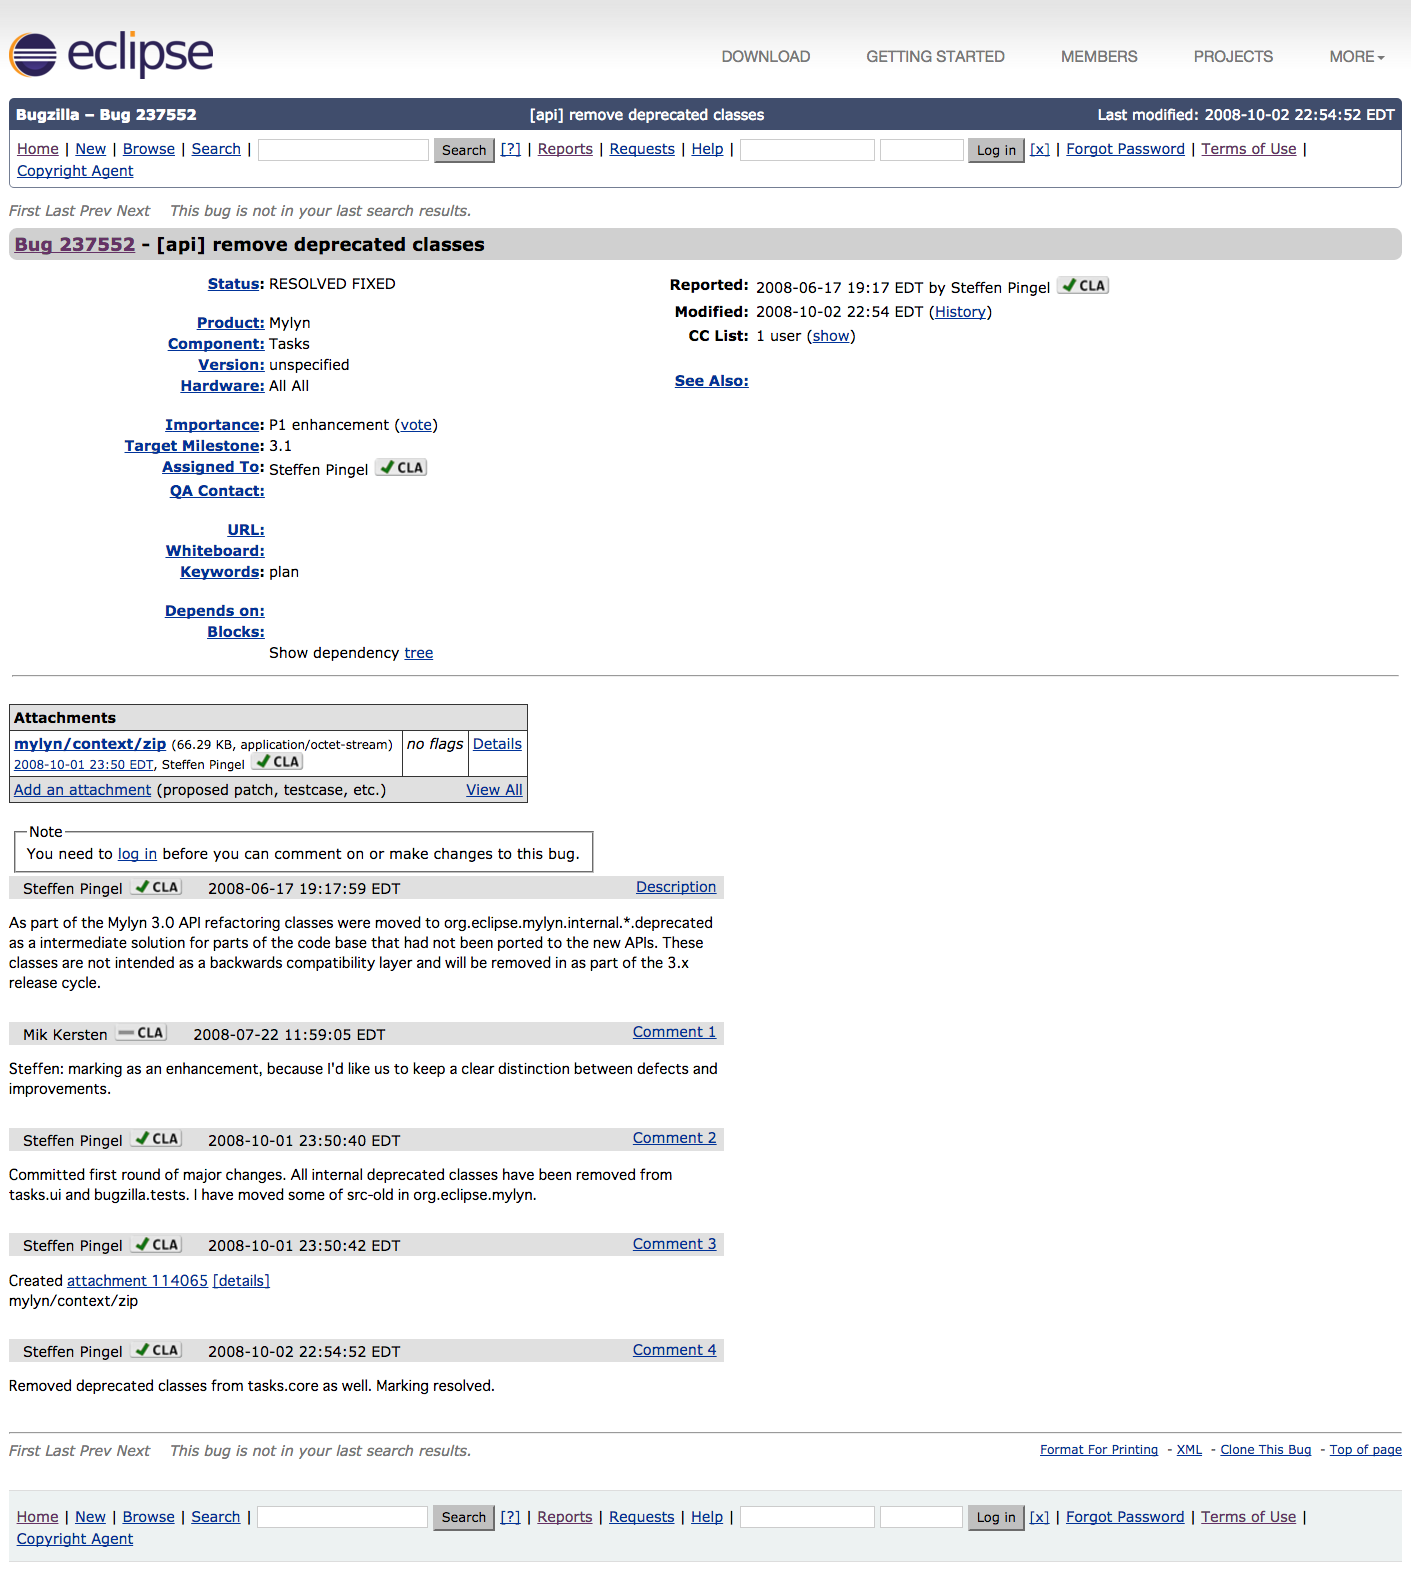
\includegraphics[width = \linewidth]{resource/bugzilla_webpage.png}
  \caption{MylynログがアップロードされているBugzillaのページの例 (\url{https://bugs.eclipse.org/bugs/show_bug.cgi?id=237552})}
  \label{bugzilla_webpage}
\end{figure}


操作イベントはXMLの要素で表され、{\it Kind}、{\it StructureHandle}などの属性が存在する。
以下の節ではそれぞれの属性について詳しく説明する。

\section{Kind}\label{kind_sec}
{\it Kind}属性はすべての操作イベントに対して記録され、イベントの種類を表している。
{\it Kind}のリストを表\ref{kind_table}に表す。
表に含まれる{\it Kind}のうち、``command"、``preference"、``attention"の3つは、Mylynが内部的に持っているのみでファイルには書き出されない。

先行研究\cite{6233415,KatoJapanese:2011,ss2012-76,ss2013-84,Yamamori:2016}の手法では変更を伴う操作と変更を伴わない操作を区別する必要があるが、Mylynログにはこの情報が記録されていないため、Mylynログをこれらの手法に適用することは出来ない(図 \ref{mylyn_interaction})。

本稿においては、エディタのカーソル位置を開発者が閲覧しているコードとみなせることから、{\it Kind}が``edit"であるような操作イベントは開発者がコードを閲覧していると解釈し、そのような操作イベントを利用して開発者が閲覧しているコードを特定する。
また、{\it Kind}が``edit"以外である操作イベントは本稿では利用しない。

\begin{table}[tb]
  \centering
  \caption{Mylynによって記録される{\it Kind}の一覧}
  \label{kind_table}
\begin{tabular}{ll}
  \hline
  Kind & 概要\\
  \hline
  selection & ファイルオープン、タブ切り替え\\
  edit & エディタ上でのカーソル位置 (コードをエディットしたかどうかを問わない)\\
  propagation & パッケージエクスプローラー上での成果物名のクリック操作\\
  command & ボタンのクリック、 キーショートカットの実行など\\
  preference & ワークベンチの設定の変更\\
  prediction & 開発者が行う可能性のある操作の予測\cite{Kersten:2006}\\
  manipulation & Mylynのタスクコンテクストに手動で成果物を追加する操作\\
  attention & タスクの活性化と非活性化\\
  \hline
\end{tabular}
\end{table}

\section{Date}\label{date_sec}
操作イベントには、"{\it StartDate}","{\it EndDate}"の2つの時間に関する属性がある。
これらはそれぞれ、タスクを活性化させている期間全体での最初のタイムスタンプと最後タイムスタンプを表現している。
操作履歴がMylynログに出力される際、開発者の操作は、成果物名と{\it Kind}の組に対して1つの操作イベントに集約される(図\ref{mylyn_interaction})。
この集約機能により、開発者が実際に成果物を閲覧した正確な時間や順序の情報は欠落してしまい、復元することができなくなる。
図\ref{mylyn_interaction}を例にとり、開発者が「$A\ra C \ra A \ra B \ra C \ra A$」の順にファイルを閲覧した場合を考える。
この場合、Mylynログにはそれぞれの成果物を閲覧した最初の時刻と最後の時刻が{\it StartDate},{\it EndDate}であり{\it Kind}が``edit"であるような操作イベントが記録される。
この操作イベントから、もとの閲覧順序を復元することはできなくなっている。
したがって、成果物への操作の順序が重要である先行研究\cite{6233415,KatoJapanese:2011,ss2012-76,ss2013-84,Yamamori:2016}の手法にMylynの操作履歴を適用することは出来ない。
\begin{figure}[tb]
  \centering
  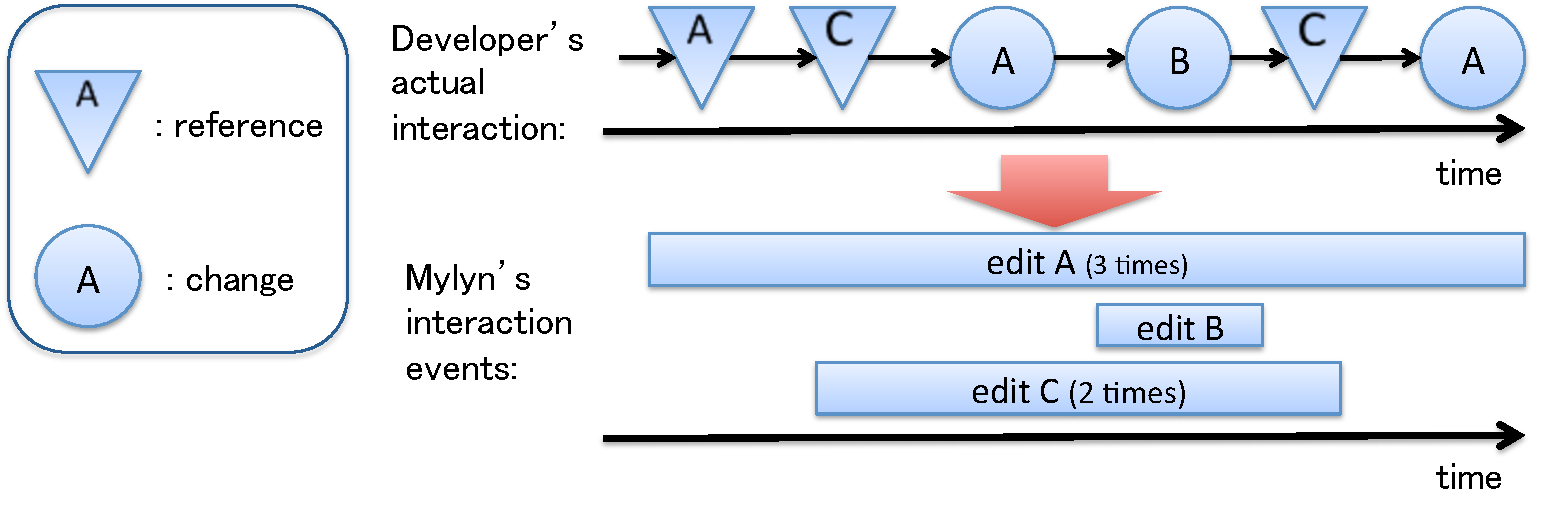
\includegraphics[width = \linewidth]{resource/mylyn_interaction.pdf}
  \caption{Mylynで記録される操作イベントの概略}
  \label{mylyn_interaction}
\end{figure}
\section{StructureHandle}
{\it StructureHandle}は操作イベント発生時に操作されたソフトウェア成果物を表す属性であり、すべての操作イベントに記録される。
{\it StructureHandle}には、``Java要素"、``jarファイルに含まれるJava要素"、``その他の要素"の3つの種類が存在する。
これらの3つの種類の成果物は、{\it StructureHandle}の文字列表現のフォーマットがそれぞれ異なる。

Java要素についてはMylynのオリジナルのフォーマッティングルールが適用され、プロジェクト、パッケージ、ファイル、クラス、メソッド、フィールドのうちのいずれかの粒度で記録される。
ここで、Mylynによって記録される成果物の粒度は各操作に対し1つのみであることに注意が必要である。
例えば、ある操作イベントがコード上のメソッドブロック内で発生した場合、この操作はメソッドの粒度のみで記録され、このメソッドを含むクラス、ファイル、パッケージ、プロジェクトの粒度では記録されない。
したがって、クラスに対する操作イベントは、メソッドブロックまたはフィールド行以外の部分で操作イベント発生した時のみ記録され、同様にファイルに対する操作イベントは、クラスブロックの外で操作イベントが発生した場合のみに記録される。

Java要素を表す{\it StructureHandle}の例として、``=W/src$<$X\{Y.java[Y$\sim$z$\sim$I"という{\it StructureHandle}を考える。
\begin{comment}
]%Vimプラグインが暴れないためのおまじない
\end{comment}
これは、「{\it z(int arg)}」という名前のメソッドが操作されたことと、このメソッドが、「{\it W}プロジェクトの中の{\it src}というソールフォルダ内にある{\it X}パッケージの{\it Y.java}というソースファイルの{\it Y}クラス」内にあることを示す。
引数の{\it I}の部分はEclipseのSignatureシンタックス\footnote{\url{http://help.eclipse.org/mars/topic/org.eclipse.jdt.doc.isv/reference/api/org/eclipse/jdt/core/Signature.html}}である。

jarファイルに含まれるJava要素については、通常のJava要素と似たフォーマッティングルールで記録される。
その他のファイルについては、プロジェクトルートの相対パスが"/"区切りでそのまま記録される。

本稿では、\ref{experiment_chap}章の実験においては、{\it StructureHandle}が通常のJava要素を表し、かつファイルレベルまたはメソッドレベルであるような操作イベントのみを用いる。

\section{NumEvent}
{\it NumEvent}は、集約した操作イベントの個数を表す数値であり、Mylyn 3.0.3で導入された。

Mylynの内部では操作イベントが頻繁に発生している。
{\it Kind}が``edit"である操作イベントは、開発者が「エディタ上でカーソルを動かした後カーソルを一定時間(1秒程度)止める」という動作を行なうたびに発生する。
Mylynではこのように発生した操作イベントを1つに集約する際、いくつの操作イベントを集約したかを{\it NumEvent}という属性で記録している(図\ref{mylyn_interaction})。
\section{Interest}
{\it Interest}とは、Mylynエンジンが計算する成果物に対する開発者の興味の度合い(Degree of Interest, DoI)であり\cite{Kersten:2006}、少なくともMylynの最初のメジャーリリースより前の時点で実装されたものである。
この属性は、対象とする成果物を操作するたびに急激に増加し、対象とする成果物以外を操作するとゆるやかに減少するような指標であり、
「タスクに関係する成果物の集約」というMylynの主機能の実現のために使われている。

\chapter{Mylynの操作履歴を細粒度にする拡張}\label{mylynplus_chap}
\section{概要}
本章では、開発者が変更を行なったかどうかを検知する機能と、変更情報と時系列情報を操作の属性として加えてMylynログに出力する機能をMylynに加える拡張について述べる。

多くの操作履歴収集ツール(表\ref{finegrained})は、操作の順序や変更の有無の情報などを含む細粒度の操作履歴を取得することができ、これらの情報を用いた変更支援手法の研究では一定の成果を上げている。
しかし、これらの操作履歴取得ツールは一般に普及しておらず、
実証実験に用いるためのデータセットを収集することが困難である。
\cite{6233415,KatoJapanese:2011,ss2012-76,ss2013-84,Yamamori:2016}ではデータセット収集のために、15人の被験者に対し2週間程度の開発を行わせることで操作履歴を取得しているが、人数、期間が小さいことや実製品の開発で取得した操作履歴ではないことから、より一般的なデータセットを利用する必要がある。

一方、Mylyn\cite{Kersten:2005}は一般の開発者に配布されているタスクマネジメントツールであり、操作履歴の取得が可能である。
MylynはEclipseに標準でインストールされており、Mylyn自身の開発プロジェクトにおいて現在までに7年分の操作履歴が記録されているなど多くの開発プロジェクトでMylynが使われていることから、この操作履歴を利用することでより一般的な実証実験を行なうことが可能となる。
しかし、Mylynの記録する操作履歴(Mylynログ)は操作の順序(\ref{date_sec}節)や変更の有無(\ref{kind_sec}節)が記録されておらず、既存の変更支援手法にこの操作履歴を適用することが出来ない。

Mylynログを用いて既存の変更支援手法を実施するために、Mylynの出力する操作履歴に細粒度の情報を付け加える拡張を行なうことを考える。
これを実施することで、既に広く配布されているMylynプラグインを利用しているプロジェクトにおいて、より長期間、大人数、かつ実製品の開発で記録された細粒度操作履歴を取得できるようになる。

\section{設計}
Mylynに対して次の3点の拡張を行なうことで、前節で述べた情報をMylynログに加える。
\begin{enumerate}
  \item 変更を伴う操作かどうかの情報を記録する
  \item カーソルがある成果物から別の成果物に移るたびに、カーソルが成果物の中に入った時刻、出た時刻の情報と、この期間に変更を伴ったかどうかを記録する
  \item {\it Kind}が"edit"である操作イベントに以上の情報を加えて、ファイルに出力する
\end{enumerate}
\subsection{変更を伴う操作かどうかの情報を記録する}
機能1は、{\it Kind}が"edit"である操作イベントが発生するたびにその成果物が含まれているファイルの内容を取得し、直前の操作イベントと比べファイルの内容が変化していた場合は「変更した("modified")」、そうでない場合は「参照した("referred")」として操作イベントに情報を付け加えるで実現した。
ただし、直前の操作イベントと比べ成果物名({\it StructureHandle})が変化していた場合はカーソルが成果物間を移動したことを示しているため、ファイルの内容の変化にかかわらず「参照した」扱いとする。
また、Mylynのタスクを活性化した直後の操作イベントは、直前の操作イベントがないため「参照した」扱いとする。

ファイルを保存する前のファイルの内容を取得する必要があるため、ファイルの内容の取得はファイルシステムからではなく、Eclipseのエディターから取得している。
また、ファイルの比較は変更されたかどうかの2択で良いため、ファイルの内容をJavaのStrint\#hashCode()メソッド\footnote{\url{https://docs.oracle.com/javase/8/docs/api/java/lang/String.html\#hashCode--}}でハッシュ化してから比較して、高速化を図った。

\subsection{カーソルが成果物の中に入った時刻、出た時刻の情報と、この期間に変更を伴ったかどうかを記録する}
機能2のうち時刻については、{\it Kind}が"edit"である操作イベントが発生するたびに直前の操作イベントの成果物名を比較し、変化していた場合は、直前の操作イベントの時刻を直前の操作イベントの成果物からカーソルが離れた時刻、今発生した操作イベントの時刻をその成果物にカーソルが入った時刻として記録することで実現する。
ただし、Mylynのタスクを活性化した直後の操作イベントは、直前の操作イベントがないためカーソルが成果物に入った時刻のみを記録する。
さらに、Mylynが非活性化した時は、直前の操作イベントの成果物からカーソルが離れたとみなしてその時刻を記録する。

機能2のうち変更を伴ったかどうかについては、カーソルが成果物に入った時刻から出た時刻までの間に「変更した」と記録されている操作イベントが1つでも存在する場合は「変更した」、すべての操作イベントが「参照した」ならば「参照した」とすることで実現する。

\subsection{ファイルに出力する}
機能3では、Mylynログに操作履歴を書き出す際にInteractionEventという要素に{\it DurationList}という属性を追加し、その属性値として機能2で得た情報を書き込むことで実現する。

MylynログはMylynプラグイン自身の動作に不可欠であるほか、他のEcilpseプラグインに使われている可能性があり、また、関連研究(\ref{coarse_sec}節)などのようにMylynログを研究対象としている研究もあり、大きくXMLの形式を変更して後方互換性を失うことは出来ない。
そのため、本拡張ではMylynログのXMLに新しい要素を追加することはせず、InteractionEventという操作イベントを表す要素に新しく1つ属性を増やすのみに留めることで、XMLの形式の変更を最小限にして、後方互換性を高めている。

{\it DurationList}の形式をEBNF記法\footnote{\url{http://www.cl.cam.ac.uk/~mgk25/iso-14977.pdf}}で以下に示す。
\begin{verbatim}
  DurationList = "[" , { Duration , "," } , Duration , "]" ;
  Duration = Date , "/" Date , "/" , Ismodified ;
  Date = "(yyyy-MM-dd HH:mm:ss.S zの形式で表現された時刻)" ;
  Ismodified = "modified" | "referred" ;
\end{verbatim}
ここで、\texttt{Duration}に含まれる2つの\texttt{Date}のうち、1つ目はカーソルが成果物に入った時刻を、2つ目はカーソルが成果物から出た時刻を表す。
また、\texttt{DurationList}は\texttt{Duration}を時系列順に並べたものである。


属性を追加して情報を書き込む欠点として、DurationListが\{開始時刻,終了時刻,変更の有無\}の3つ組をリストにしたものであるのに、これらの情報がXMLのシンタックスに含まれないことである。
そのため、DurationListの情報を利用する場合は、XMLの解析器を用いてDurationListを抜き出したのち、さらに上記のEBNF記法による文法に基づきDurationListの内容をトークン分解する必要がある。
この点については、DurationListの情報の利用者が現状では本論文の著者とその研究グループのみになると考えられるため許容できるとした。

\section{実行例}
本拡張によって記録されるMylynログの例として、著者が\ref{experiment_chap}章で実装した実験コードを編集する際に記録したMylynログから、{\it DurationList}が含まれるInteractionEventのうち2つをリスト\ref{durationlist_fig}に示す。
なお、このMylynログ全体は付録\ref{mylyn_log_appendix}に掲載する。

\begin{lstlisting}[float, floatplacement=tb, style=normalsize, language=xml, caption=拡張されたMylynによって記録されたMylynログの例(ただしXML上で実体参照に変換された文字はもとに戻している), label=durationlist_fig]
<InteractionEvent Delta="null" EndDate="2016-01-12 17:03:06.423 JST" Interest="15.0" Kind="edit" Navigation="null" OriginId="org.eclipse.jdt.ui.CompilationUnitEditor" StartDate="2016-01-12 16:38:31.648 JST" StructureHandle="=MylynGitPrediction/src<tkobaya.yamamori.mgprediction.combine{MylynReaderResult.java[MylynReaderResult~ addInteractionSet~QMylynInteractionHistory;~D" StructureKind="java" NumEvents="15" CreationCount="103" DurationList= "[2016-01-12 16:38:31.648 JST/2016-01-12 16:40:16.482 JST/modified, 2016-01-12 17:02:58.409 JST/2016-01-12 17:03:06.423 JST/modified]"/>
<InteractionEvent Delta="null" EndDate="2016-01-12 16:52:53.826 JST" Interest="29.0" Kind="edit" Navigation="null" OriginId="org.eclipse.jdt.ui.CompilationUnitEditor" StartDate="2016-01-12 16:43:09.833 JST" StructureHandle="= MylynGitPrediction/src<tkobaya.yamamori.mgprediction.combine{SingleFileSet.java[SingleFileSet~putAll~QMap<+QInteger;+QDouble;>;" StructureKind="java" NumEvents="29" CreationCount="157" DurationList=" [2016-01-12 16:43:09.833 JST/2016-01-12 16:43:11.666 JST/referred, 2016-01-12 16:51:14.131 JST/2016-01-12 16:51:14.131 JST/referred, 2016-01-12 16:51:38.25 JST/2016-01-12 16:52:53.826 JST/modified]"/>
\end{lstlisting}
\begin{comment}
]}]} //おまじない
\end{comment}

1つ目の操作イベントは、{\it Kind}が"edit"であることからカーソル移動に関する操作があったことがわかり、
{\it StructureHandle}から、"MylynGitPrecition"というプロジェクトの中にある\newline"tkobaya.yamamori.mgprediction.combine"パッケージの"MylynReaderResult.java"に実装されている"MylynReaderResult\#addInteractionSet( MylynInteractionHistory a, double b)
\footnote{メソッドの仮引数名は記録されないため、ここではa, b, \dots とする}"というメソッドに対する操作であることがわかる。
また、{\it StartDate}と{\it EndDate}からこのメソッドは2016年1月12日16時38分31秒648(日本標準時)に初めてカーソルが入り、同日の17時3分6秒423を最後にカーソルがこのメソッドに入ることはなかったことがわかる。
同様に2つ目の操作イベントは、"SingleFileSet\#putAll( Map<Integer,Double> a)"というメソッドにカーソルが入ったことを表し、その最初の時刻は16時43分09秒833、最後の時刻は16時52分53秒826であった。
したがって、以上のDurationListを含まない情報からこれらのメソッドは16時43分から53分ごろまでの10分間はどちらもカーソルが入っていた可能性がある。
しかし、この情報のみでは、2つのメソッドにカーソルが入った順番の情報を復元することが出来ない(図\ref{only_startdate_enddate})。

\begin{figure}[tb]
  \centering
  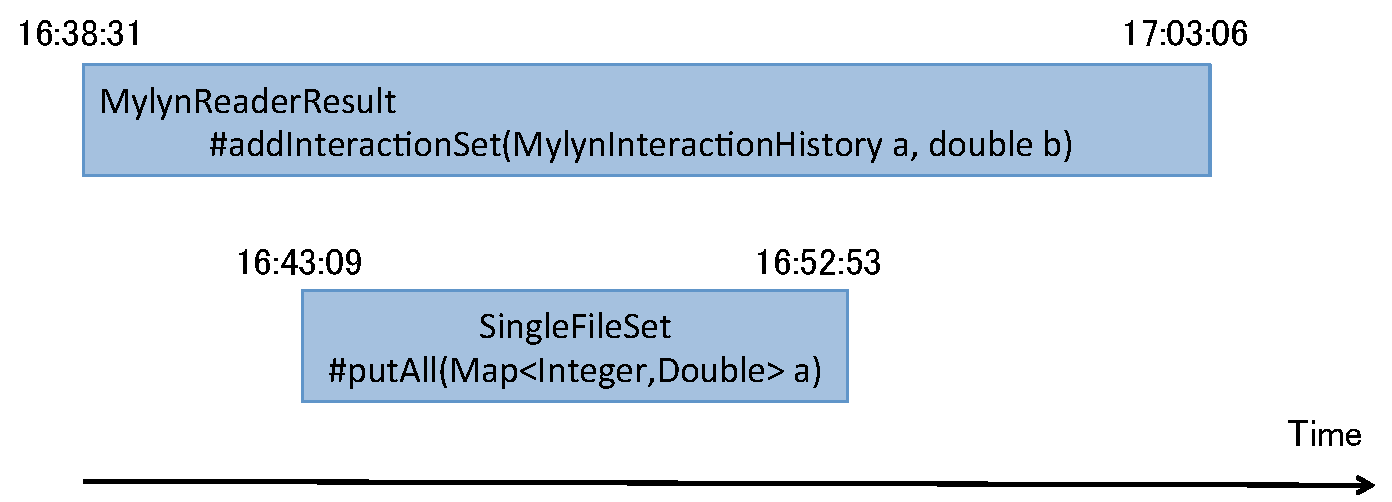
\includegraphics[width = \linewidth]{resource/only_startdate_enddate.pdf}
  \caption{拡張前のMylynログでは、カーソルの移動した順序を復元することが出来ない}
  \label{only_startdate_enddate}
\end{figure}


本拡張で追加した{\it DurationList}について注目すると、"addInteractionSet()"メソッドには16時38分31.648秒〜16時40分16秒482と17時2分58秒409〜17時3分6秒423の2回カーソルが入っており、
"putAll()"には16時43分9秒833〜16時43分11秒666と、16時51分14秒131、16時51分38秒〜16時52分53秒826の3回カーソルが入ったことがわかる。
したがって、これら2つのメソッドのみについて考えると、カーソルの移動した順序は
"addInteractionSet()" $\Ra$
"putAll()" (3回) $\Ra$
"addInteractionSet()"
であることがわかる(図\ref{with_durationlist})。

また、カーソルが入ってから出るまでに変更を伴ったかどうかについても記録されており、"addInteractionSet()"の2回のカーソル移動では変更を伴っていること、"putAll()"の3回のカーソル移動のうち、1回目2回目は変更が行われておらず、3回目のみ変更が行われていることがわかる(図\ref{with_durationlist})。

\begin{figure}[tb]
  \centering
  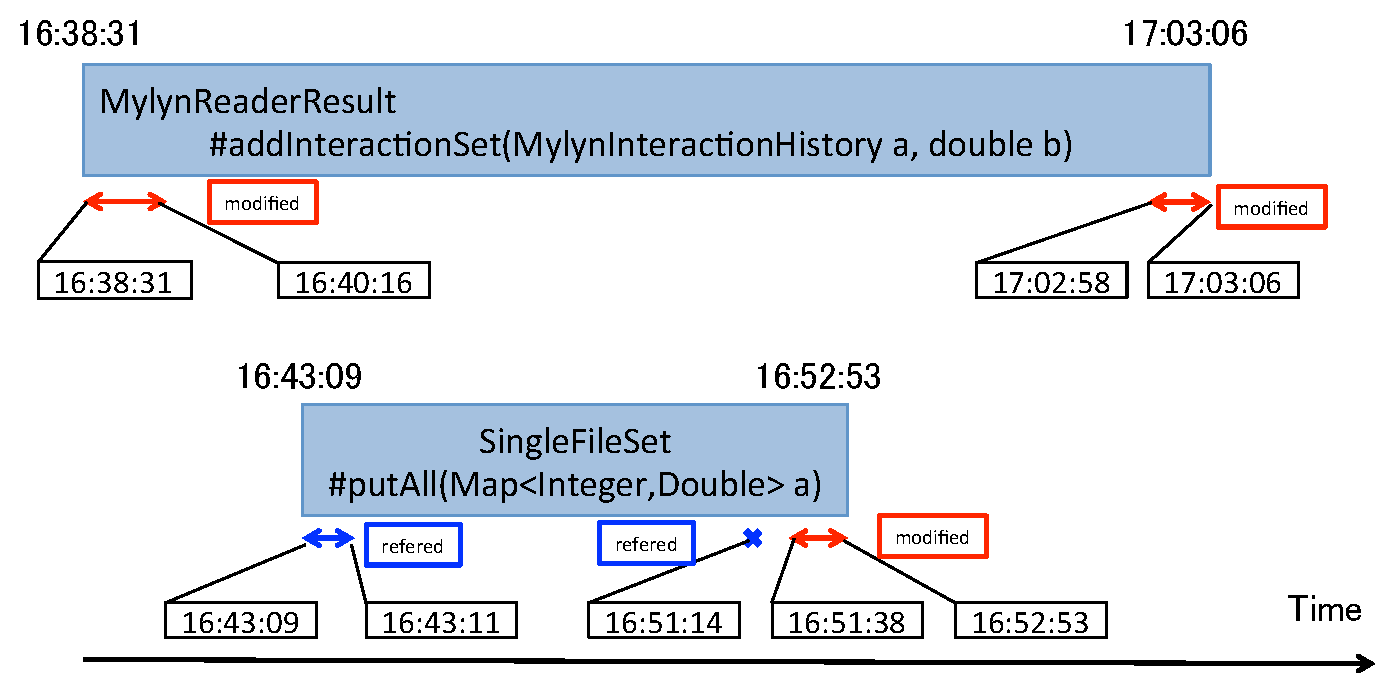
\includegraphics[width = \linewidth]{resource/with_durationlist.pdf}
  \caption{拡張後のMylynログでは、カーソルの移動した順序を復元でき、変更の有無も記録される}
  \label{with_durationlist}
\end{figure}

以上のようなMylynの拡張を行なうことで、
\cite{6233415,KatoJapanese:2011,ss2012-76,ss2013-84,Yamamori:2016}の手法に対してMylynログを適用することができるようになる。

\chapter{Mylynの操作履歴による変更推薦}\label{experiment_chap}
\section{概要}
\ref{mylynplus_chap}章では、今後記録されるMylynログに細粒度な操作の情報を付け足すことで、既存の細粒度操作履歴を用いる変更支援手法にMylynログを適用するアプローチを採用した。
本章では、Mylynログに細粒度な情報を付け足すことなく、これまでに記録されたMylynログを用いて変更支援を行なえるかどうかを調査する。

Mylynの操作履歴は\ref{date_sec}節で述べたように時間の情報が不完全であり、\ref{kind_sec}節で述べたように変更と参照の情報が含まれていない。
これらの情報を擬似的に復元するために、Mylynの操作履歴をGitの改版履歴と突合し、擬似的に細粒度操作履歴を作成する。
このようにして得られた操作履歴はGitのコミットの時刻を用いて時間の情報が復元され、またコミットに含まれるファイルやメソッドの情報をもとに変更と参照の情報が復元される。
そして、この擬似細粒度操作履歴を既存の改版履歴ベースの変更推薦手法に適用することで、Mylynの操作履歴が変更推薦に適用できるか否かを検証する。
検証の際は、既存の改版履歴ベースの変更推薦手法に改版履歴を適用する従来の手法を比較対象とし、推薦精度が向上しているかを確認する。

実証実験は以下の4段階で行なう(図\ref{procedure})。
\begin{enumerate}
  \item 改版履歴と操作履歴を取得する(\ref{obtainhistory_sec}節)
  \item 得られた改版履歴と操作履歴を突合する(\ref{joining_sec}節)
  \item 相関ルールを抽出する(\ref{extractrules_sec}節)
  \item 変更推薦を行なう(\ref{ranking_sec}節)
  \item メトリクスを用いて相関ルールの質を評価する(\ref{metrics_sec}節)
\end{enumerate}
\begin{figure}[tb]
  \centering
  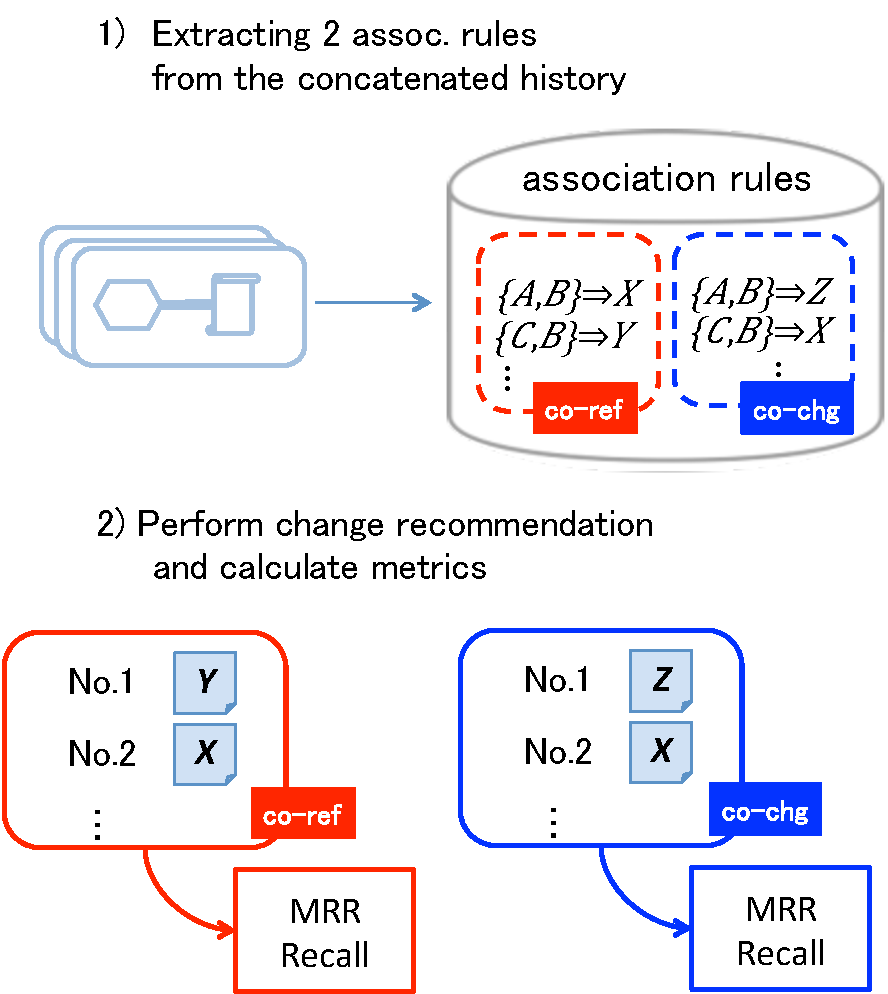
\includegraphics[width = \linewidth]{resource/procedure.pdf}
  \caption{実証実験の手順}
  \label{procedure}
\end{figure}

\section{改版履歴と操作履歴の取得}\label{obtainhistory_sec}
まず、Gitリポジトリの改版履歴に含まれる全てのコミットから変更されたファイル、変更されたメソッドの2つのリストを抽出する。

開発者がEGitというGit操作を行なうEclipseプラグインを利用してリポジトリにコミットしていた場合、EGitは活性化中のMylynタスクのBug IDをコミットメッセージに自動的に加える機能がある。
Bug IDの情報がコミットメッセージに含まれている場合は、この情報をコミットと共に保存する。

次に、EclipseプロジェクトのBugzillaウェブサイト\footnote{\url{https://bugs.eclipse.org/bugs/}}のバグ詳細ページをクローリングし、アップロードされている全てのMylynログを取得する。
Mylynログは\ref{mylyn_chap}で述べたようにBugzillaのバグ詳細ページにアップロードされており、バグ詳細ページは\texttt{http://bugs.eclipse.org/bugs/show\_bug.cgi?id=(整数)}で表されるURLなので、整数の部分を1〜400000まで動かして一斉取得することができる。
さらに、Bugzillaのバグ詳細ページから、活性化していたMylynタスクのBug IDと、Mylynログがアップロードされた時刻、アップロードした開発者の名前の、3つの情報を取得し、ダウンロードしたMylynログに紐付けて記録する。

得られたMylynログから、{\it Kind}が"edit"であるような操作イベントを抜き出し、そのうちファイルレベルの操作イベントとメソッドレベルの操作イベントの2つのリストを抽出する。
本章では、Mylynログに含まれる操作された要素のリストを、Gitリポジトリにおけるコミットと同様に{\bf セッション}と呼ぶ。

コミットから変更されたメソッドの情報を抽出する際は、Kataribe (Historage)\cite{Hata:2011,Fujiwara:2014}というツールを使用した。

得られたMylynログはEclipseの約300プロジェクト\footnote{\url{https://projects.eclipse.org/}}のいずれかの開発で記録されたものであるが、そのほとんどがMylynプロジェクトおよびそのサブプロジェクトであった。
そのため、本章の実証実験の対象リポジトリはMylynプロジェクトに含まれる12リポジトリをGitHub\footnote{\url{https://github.com/eclipse?query=mylyn}}とした(12リポジトリの詳細は付録\ref{mylyn_repo_appendix}を参照)。
また、Bugzillaへのクローリングの結果、6270のバグ詳細ページから8156のMylynログをダウンロードした。

\section{改版履歴と操作履歴の結合}\label{joining_sec}
改版履歴のコミットと操作履歴のセッションについて、同じ開発活動で作成されたと考えられるもの同士を紐付け、結合した履歴を作成する。

Mylynログは、Bug ID毎に作成されるが、セッションに対応するコミットの情報はMylynログにもBug IDにも含まれていない。
本稿においては、同じ開発活動で作成されたコミットとセッションは、以下の1)〜3)が成り立つと考え、これらをコミットとセッションを紐付ける際の条件とした(図\ref{concat_figure})。
\begin{enumerate}
  \item Bug IDが同じであること
  \item 著者名が同じであること
  \item 作成日時の差が2分以内であること
\end{enumerate}
\begin{figure}[tb]
  \centering
  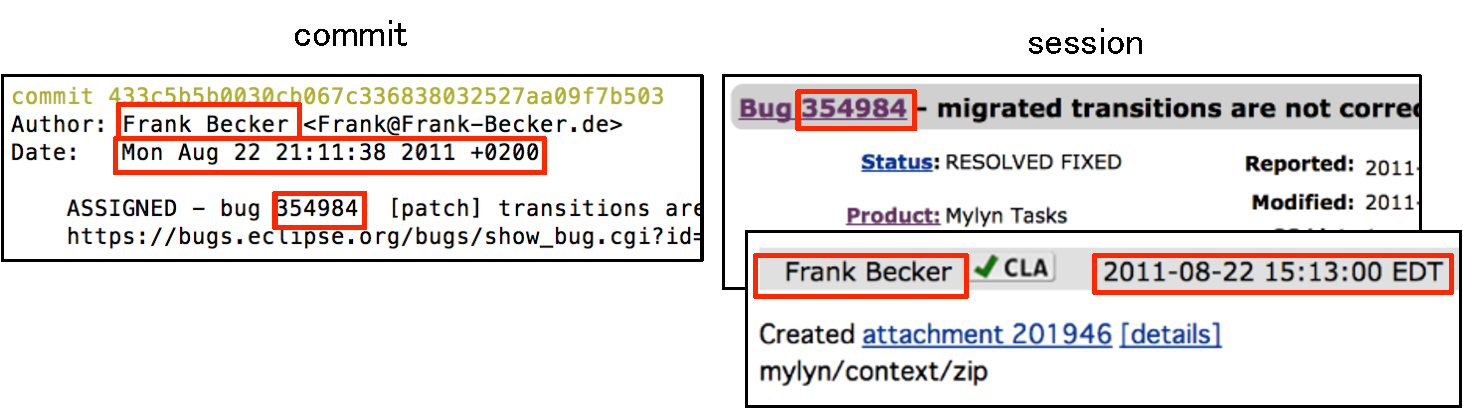
\includegraphics[width = \linewidth]{resource/concatenating.pdf}
  \caption{1)Bug ID、 2)アカウント名、3) 作成日時の差が2分以内であるの1)〜3)を条件に、コミットとセッションを結合する}
  \label{concat_figure}
\end{figure}
このうち、2)の条件については、GitはGitクライアントのアカウント名を、MylynはBugzillaのアカウント名を利用する。
しかし、これらのアカウント名が異なる開発者が多く存在した(例えば、Bugzillaのアカウント名が"Steffen Pingel"の開発者と、Gitクライアントのアカウント名が"spingel"の開発者は、アカウント名が異なるが同一人物と考えられる)。
そのため、アカウントリストを人手で判別することによりこれらのアカウント名の対応関係のリストを作成し、2)の条件に利用した。
最終的に、38のGitのアカウント名のうち、18名については対応するBugzillaアカウントを見つけることに成功した(表\ref{transaction})。
半数以上のGitのアカウント名の対応関係を見つけることができなかったが、これは以下のことが原因であると考えられる。
\begin{itemize}
  \item 開発者が、Mylyn開発時の義務(\ref{mylyn_chap}章参照)を果たさず、Mylynログをアップロードしていなかったため
  \item 「実名」と「よく知られているニックネーム」など、開発者がGitとBugzillaの間で相違する名前を使用していたため
\end{itemize}

3)の条件については、開発者がEGitというGit操作を行なうEclipseプラグインを利用してリポジトリにコミットしていることを仮定している。
MylynにはEGitと協調してEGitでコミットを行なった際に同時にMylynログをBugzillaに送信する機能があり\footnote{\url{https://wiki.eclipse.org/Mylyn/Contributor_Reference\#Connect_to_Gerrit_and_Git}}、この機能を開発者が利用しているならば、EGitのコミット時刻とほぼ同時刻にMylynログがBugzillaにアップロードされる。
したがって、2分という短い時間の間に作成されたコミットとセッションは、この機能を利用している可能性が極めて高く、本稿においてはこのような場合のみ同じ開発作業で作成されたコミット、セッションの可能性があるとした。

コミットとセッションの結合の結果、12のGitリポジトリに含まれるコミットと、全てのEclipseプロジェクトに含まれるセッションを結合し、968個のファイルレベルのコミット-セッションペアを得た。
結合作業後、結合されなかったコミットとセッションは実験対象から除外した。

一般に、あるGitリポジトリ中のコミットに他のリポジトリに含まれているファイルが入っていることはないが、Mylynログに含まれるセッションは、同時にEclipse上で開かれているファイル同士であれば、リポジトリをまたいだ2つ以上のファイルが同じセッションに含まれている場合もある。
しかし、操作履歴と改版履歴を用いた変更支援手法を比較するため、実証実験を行なう際は1つのGitリポジトリを実験対象とする。
対象とするリポジトリは最も多くのコミット-セッションペアを生成できた{\it mylyn.tasks}\footnote{\url{https://github.com/eclipse/mylyn.tasks}}リポジトリとした。
このリポジトリには41個のEclipseプロジェクトが含まれていた。

{\it mylyn.tasks}リポジトリに含まれる8548コミットとMylynログに含まれる8156セッションから、ファイルレベルのコミット-セッションペアが600個、メソッドレベルのコミット-セッションペアが553個生成された(表\ref{transaction})。
メソッドレベルのコミット-セッションペアの数がファイルレベルに比べて少ないが、これは、メソッドブロック内で変更が行われず、コメントやフィールド、インポート等メソッドブロック以外の部分で変更が行われたコミットが存在するためである。
このようなコミットでは、ファイルの変更は記録されるが、メソッドは変更されていない。
\begin{table}[tb]
  \begin{center}
    \caption{トランザクション数とアカウント数}
\label{transaction}
\begin{tabular}{lrr}
  \hline
  履歴の種類 & トランザクション数 & アカウント数\\
  \hline
  ({\it mylyn.tasks}の)コミット & 8548 &38\\
  セッション & 8156 &277\\
  \hline
  ファイルレベルのコミット-セッションペア & 600 & 18\\
  メソッドレベルのコミット-セッションペア & 553 & 18\\
  \hline
\end{tabular}
  \end{center}
\end{table}

一部のコミット-セッションペアは1対1対応となっておらず、ファイルレベルでは11個のペアが、メソッドレベルでは10個のペアが、1対2、1対3、2対1などの対応関係になっていた。
これは、ペアに含まれているコミットとセッションが2分以内に作成されている場合に起きるものであり、このようなペアに含まれるコミットやセッションは1つのコミットやセッションにみなせるものと考え、他のペアと同じ扱いとした。
\begin{table}[tb]
  \begin{center}
    \caption{コミット-セッションペアの対応関係}
\label{squash}
\begin{tabular}{c|rr}
  \hline
  コミット数 vs. セッション数 & ファイルレベルのペア&\# メソッドレベルのペア\\
    \hline
  1 vs. 1 & 589 & 543\\
  1 vs. 2 & 1 & 1\\
  2 vs. 1 & 9 & 9\\
  3 vs. 1 & 1 & 0\\
\hline
  合計 & 600& 553\\
  \hline
\end{tabular}
  \end{center}
\end{table}

\begin{figure*}[tb]
  \centering
  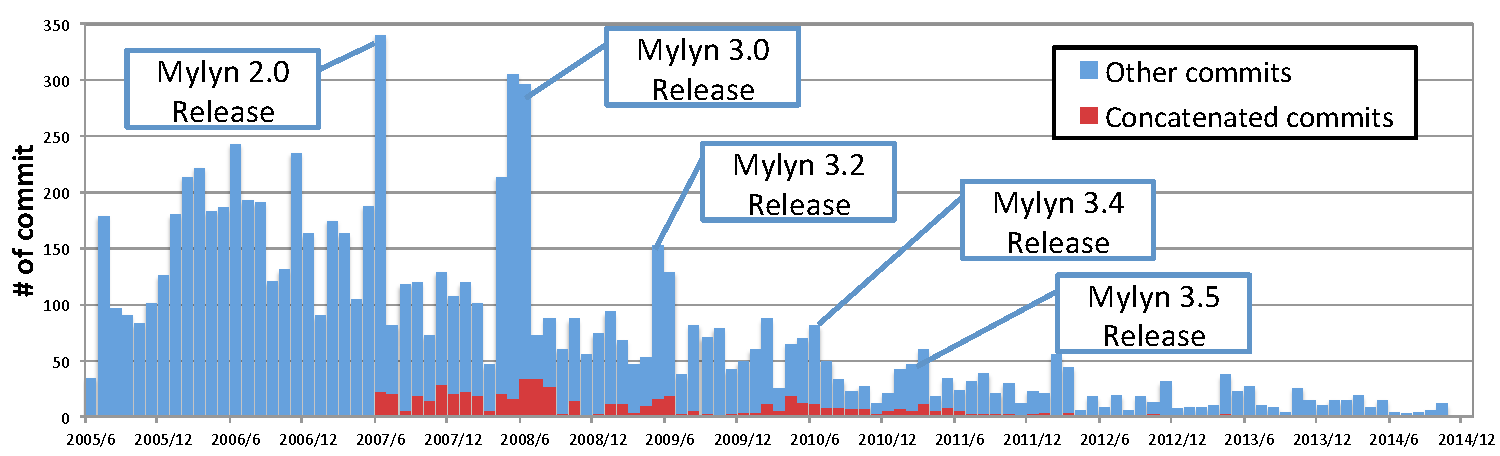
\includegraphics[width = 0.9\linewidth]{resource/commit_distribution.pdf}
  \caption{全てのコミットと、ファイルレベルでセッションと結合できたコミットの作成時刻の分布}
  \label{commit_distribution}
\end{figure*}
図\ref{commit_distribution}は、ファイルレベルにおける、セッションと結合できたコミットの作成時刻の分布である。

セッションと結合できたコミットは2007年6月に初めて出現したが、これはMylyn 2.0のリリース時期と一致している。
この時期からMylynの開発者はメンテナンスタスクの際にMylynログを継続的にアップロードするようになり、結合されたコミットはいくつかのメジャーリリースを跨いで分布していることがわかる。
したがって、今回取得できたコミット-セッションペアを利用して変更推薦を行なうことで、変更推薦の一般的な特徴を議論することが可能となる。

一般に、コードの変更を行なった場合、そのコードをエディタ上に表示するためにコードの参照を同時に行なっているはずであり、この仮定に基づくならばGitのコミットに含まれている成果物はMylynのセッショに含まれている成果物の部分集合となるべきである。
しかし、この仮定に反し、ファイルレベルの600個のコミット-セッションペアのうち19\%はこのような条件が成り立たず、コミットに含まれていてセッションに含まれないファイルが存在した。
この事実に対応する仮定として、セッションに含まれていないがコミットに含まれている成果物は、実際は参照されていたが、操作としてMylynが記録することができなかった場合について考える。
この状況は、開発者がMylynタスクを活性化し忘れたままコードの変更を開始し、開発途中でMylynタスクを活性化したのち、変更したコードをMylynタスクの活性化後は一度も触らなかった場合に起こりうる。
この仮定から、コミットに含まれる全ての成果物は参照されたとみなし、参照セットをセッションとコミットの和集合、変更セットをコミットと定義することにする。
\begin{eqnarray}
  参照セット &=& コミット \cup セッション\\
  変更セット &=&  コミット
\end{eqnarray}
そして、参照セットの列を{\bf 参照履歴}、変更セットの列を{\bf 変更履歴}と定義する。
\section{相関ルールの抽出}\label{extractrules_sec}
A-prioriアルゴリズムを利用した相関ルールマイニング手法を参照履歴、変更履歴に適用して、相関ルールを抽出する。

Zimmermannらが実装したeROSE\cite{Zimmermann:2005}は、改版履歴から共変更の相関ルールを抽出し変更推薦を行なうツールである。
この共変更相関ルールはファイル同士の変更の関係を表し、以下のように定義される。
$x_1$をファイルの集合、$x_2$を1個のファイルとする。
相関ルールは$x_1 \Ra x_2$と表され、$x_1$に含まれる全ての要素が変更された場合、$x_2$も変更されることが予想できることを意味する。
$x_1$と$x_2$はそれぞれ、「左辺」、「右辺」と呼ばれている。

LCExtractor\cite{Hagward:2015,Mori:2015}も同様に改版履歴から共変更の相関ルールを計算するツールである。
LCExtractorはeROSEと異なり、成果物名の変更に追随し、現存しないファイルを含むルールを出力しないという機能がある。
本稿ではこのLCExtractorを拡張し、変更履歴や参照履歴を入力することで、共変更の相関ルール({\bf co-change association rules(co-chg)})と共参照の相関ルール({\bf co-reference association rules(co-ref)})が計算できるようにした。
特筆すべき点として、改版履歴と操作履歴を結合した参照履歴からLCExtractorを用いて共参照の相関ルールを抽出することで、LCExtractorの特徴である成果物名の変更の追従機能を利用することができる点がある。
成果物名の変更は、Mylynログのどの操作イベントにも記録されていないが、Gitのコミットには記録されているため、コミットとセッションを結合させることで変更の追従を行なうことが可能となった。
なお、\ref{metrics_sec}節で後述するように、履歴のうちの一部を学習セットに用いて他の一部を評価セットに用いるために、LCExtractorの「現存しないファイルを含むルールを出力しない機能」は本稿では使用しない。

A-prioriアルゴリズム\cite{Bondugula:2006}とは、アイテムセットのデータベースから、効率的な枝刈りを行いながら相関ルールを抽出するアルゴリズムであり、eROSEやLCExtractorの実装に使われている。
ルールの枝刈りには、支持度($support$)と確信度($\confidence$)という2つの相関ルールの評価尺度を用いる。
トランザクション集合$T$内で見つかったある相関ルール$L \Ra R$において
$support$とは全体のトランザクション数のうち$L$および$R$を含んでいるトランザクションの割合であり、
$\confidence$とは$L$を含むトランザクション数のうち$L$および$R$を含んでいるトランザクションの割合である。
これらを形式的に表すと以下のようになる。
\begin{eqnarray}
  support_{T,L \Ra R} &=& \frac{| L \cup R |}{|T|}\\
  \confidence_{T,L \Ra R} &=& \frac{| L \cup R |}{|L|}
\end{eqnarray}
なお、$minsup$については、\cite{Zimmermann:2005}のように全てのトランザクション数に対する割合ではなく、$L$および$R$を含むトランザクション数を利用している研究もある。\cite{Zimmermann:2005}ではこのような数値を{\it minimum support count}と呼んでいる。
本稿では{\it minimum support count}は使用せず、$minsup$は全トランザクション数に対する相対値を用いる。

参照履歴を用いた変更推薦の効果を測定するため、参照履歴と変更履歴の両方から相関ルールを抽出し、比較を行なう。
ルールを抽出する際、参照履歴についてはコミットと結合することができた全ての参照セットをデータセットとし、変更履歴についてはセッションと結合できたかどうかに関わらず、Mylyn 2.0のリリースが行われたコミットよりも新しい変更セットを全てデータセットとした。
Mylyn 2.0のリリース以降のコミットは、全体のコミットの63\%であった。
このとき、変更履歴についてもセッションと結合できたコミットのみを利用する方法もあったが、この方法は取得できたセッションの内容に大きくバイアスされ、参照履歴を利用した変更推薦のベースラインとしては適さない。
そのため、参照履歴と変更履歴の期間をMylyn 2.0リリース以降に揃え、期間内の全ての変更を利用することで、取得できたMylynログの内容になるべくバイアスされないよう配慮した。
ただし、以上の内容はルールを抽出する際の学習セットについてのみ適用され、評価セットについてはセッションと結合できたコミットのみを用いる。

\ref{joining_sec}節で述べたように、一般に、あるGitリポジトリ中のコミットに他のリポジトリに含まれているファイルが入っていることはないが、Mylynログに含まれるセッションは、同時にEclipse上で開かれているファイル同士であれば、リポジトリをまたいだ2つ以上のファイルが同じセッションに含まれている場合がある。
そのため、共参照の相関ルールには、対象のGitリポジトリ({\it mylyn.tasks})に含まれない成果物が含まれている可能性がある。
このようなルールのうち、対象のGitリポジトリに含まれない成果物が右辺にあるルールは変更推薦を必ず外すため、抽出したルールセットから除外する。

A-prioriアルゴリズムを利用して相関ルールを抽出する際はパラメータとしてminimum support(最小支持度, $minsup$)とminimum confidence(最小確信度, $\minconf$)を決める必要がある。
これについては\ref{setting_sec}節で述べる。

\section{変更推薦}\label{ranking_sec}
参照履歴から抽出した相関ルールと変更履歴から抽出した相関ルールをもとに、変更推薦を行なう。

相関ルールを$rule_i = (l_i,r_i)$と表す。
($l_i$,$r_i$)は相関ルール$L \Ra R$と対応し、$l_i$は左辺の成果物集合、$r_i$は右辺の成果物を表す(\ref{extractrules_sec}節参照)。
さらに、co-refの相関ルールの列を$Rule = \{rule_1, rule_2, \dots, rule_m\}$とする。
また、変更推薦を行なう対象の参照セットを$source$とする。$source$は成果物の集合である。
%また、$support((l_1,r_1)),\confidence((l_1,r_1))$を、それぞれ相関ルール$(l_1,r_1)$の$support$と$\confidence$とする。
このとき、$source$を入力として得られる変更推薦結果$recom_{Rule}(source)$は「変更推薦される成果物とそのスコアの組」のリストであり、以下のように定義する。
\begin{eqnarray}
  recom_{Rule}\left(source\right) = \bigcup_{rule_j \in Rule}
    &\left\{
    \begin{array}{ll}
      \left\{\left(r_j,score_j \right)\right\} &(\textrm{if~} l_j \subseteq source) \\
      \emptyset &(\textrm{otherwise})\\
    \end{array}
    \right.\\
    &\textrm{where}~score_j = \confidence(rule_j)\nonumber
\end{eqnarray}
$\left(r_j,score_j\right)$は成果物と数値の組であり、$r_j$は変更推薦される成果物を、$score_j$は$r_j$のスコアを表す。
また、$\confidence(rule_j)$は$rule_j$のconfidenceを返す関数である。

最終的に$recom_{Rule}(source)$の各要素$(r_j,score_j)$を$score_j$の高いものから1位、2位、$\dots$とし、成果物$r_j$の変更推薦順位とする。

この変更推薦手法は\cite{Zimmermann:2005}で提案されたものである。
ただし、\cite{Zimmermann:2005}では推薦される成果物をランキングする手法は提案されなかったため、本研究では新しく成果物にスコアをつけランキングを行なうよう手法を拡張した。

\section{評価メトリクス}\label{metrics_sec}
前節までで行なったco-refの相関ルールによる変更推薦を評価する。

ファイルレベルで600個、メソッドレベルで553個のコミット-セッションペアで評価を行なうが、この数は他の改版履歴を用いる研究と比べ比較的少ない数字である。
この少ないデータセットの中で相関ルールの効果を評価するため、コミット-セッションペアに10-分割交差検定を適用し、相関ルールの平均的な性能を確認する。
10-分割交差検定を実行する際は、コミット-セッションペアを時刻によってソートし、それぞれの区間に同じ数のペアが含まれるように区間を10分割する。
さらに、1つの区間を評価セットに、他の9つの区間を相関ルール抽出に使う学習セットに選んで変更推薦を行なうことを10区間全てで繰り返し、それぞれの区間での変更推薦の評価を平均することで、最終的な相関ルールの評価とする。
以上のような評価をco-refルールとco-chgルールで比較することで、参照履歴を用いて変更推薦を行なうことの利点や特徴について議論する。

相関ルールによる変更推薦結果の評価は、評価する変更セットに含まれる成果物を1つずつ除去し、その成果物を正しく推薦できるかを確かめることで行なう。
したがって、評価セットに含まれる各変更セットに対し、変更セットに含まれる成果物の数だけ変更推薦を適用し、それぞれの評価を平均することで、その変更セットの変更推薦時の評価とする。
この実験設定は\cite{Zimmermann:2005}の{\it error prevention}の設定と類似するものである。

評価尺度には$MRR$、$Recall$及びこれらの調和平均である$\fmeasure$を用いる。
$MRR$(平均逆順位、mean reciprocal rank)はランキングを評価するときに用いられる評価尺度であり、正しく推薦した成果物の順位の逆数を、推薦回数で平均したものである。
$MRR$は情報検索の分野で利用されているほか\cite{6233415}で変更推薦の評価を行なう際も利用されている。
$Recall$(再現度)は推薦が行われた回数を表現する尺度である。$Recall$も情報検索の分野で利用されているほか、\cite{Zimmermann:2005}で変更推薦の評価を行なう際も利用されている。

co-refの相関ルールに対するメトリクス$MRR,Recall,\fmeasure$の定義を以下に述べる。

学習セットから抽出したco-refの相関ルールを$Rule_{ref}$とする。
また評価セットの参照セットの列を$Re\!f\!erence = \{ref_1, ref_2, \dots, ref_n\}$、
評価セットの変更セットの列を$Change = \{chg_1, chg_2, \dots, chg_n\}$とする。
ここで$ref_i$と$chg_j$はそれぞれ参照セット、変更セットであり、$i=j$ならばこれらのセットは同じ開発行動を表す参照セット、変更セットである。

\ref{ranking_sec}節の$recom_{Rule}(source)$を用いて、参照セット$ref_i$に対するメトリクス$feedback_i$、$MRR_i$、 $recall_i$を以下のように定義する。
\begin{eqnarray}
   feedback_i &=& \frac{1}{|chg_i|}
  \sum_{c \in chg_i}
  \left\{
  \begin{array}{ll}
    1 ~(\textrm{if~} recom_{Rule_{ref}}(ref_i,c) \neq \emptyset)\\
    0 ~(\textrm{otherwise})\\
  \end{array}
  \right.\\
  MRR_i &=& \frac{1}{feedback_i}\frac{1}{|chg_i|}
  \sum_{c \in chg_i}
  \left\{
  \begin{array}{ll}
    getRR\left( recom_{Rule_{ref}}(ref_i,c), c \right) 
    &~(\textrm{if~} recom_{Rule_{ref}}(ref_i,c) \textrm{~contains~} c)\\
    0 &~(\textrm{otherwise})\\
  \end{array}
  \right.\\
  recall_i &=& \frac{1} {|chg_i|} \sum_{c \in chg_i}
  \left\{
  \begin{array}{ll}
    1 ~(\textrm{if~} recom_{Rule_{ref}}(ref_i,c) \textrm{~contains~} c)\\
    0 ~(\textrm{otherwise})\\
  \end{array}
  \right.\\
           &~&where~recom_{Rule}(ref_i,c) = recom_{Rule}(ref_i - \{c\})
\end{eqnarray}
ここで、$recom_{Rule}(ref_i,c)$は、$i$番目の評価セット$ref_i$と、$ref_i$に含まれる成果物$c$に対し、$ref_i$から$c$を除いた成果物集合を入力として変更推薦を行なった時の変更推薦リストである。
$getRR\left( recom_{Rule_{ref}}(ref_i,c), c \right)$は、変更推薦リスト$recom_{Rule_{ref}}(ref_i,c)$内での$c$の順位の逆数(逆順位)を返す関数である。


$Re\!f\!erence = \{ref_1, ref_2, \dots, ref_n\}$に含まれる全ての$ref_i$に対して
$MRR_i$と$recall_i$を算出し、その算術平均を最終的なメトリクス$MRR$と$Recall$とする。
加えて、$\fmeasure$を$MRR$と$Recall$の調和平均と定義する。
\begin{equation}
  \fmeasure = 2\cdot\frac{MRR \cdot Recall}{MRR+Recall}
\end{equation}

「変更推薦が行われた時の推薦精度」を算出するため、\cite{Zimmermann:2005}におけるPrecisionと同様に、$MRR_i$を算出する際に$feedback_i$を分母として用いている。
このとき、$feedback_i=0$だった(そのコミットで1度も変更推薦を行なうことがなかった)場合は、$MRR_i$自体を算出せず、$MRR$の計算対象から除外する。
一方、「変更推薦が行われたかどうかにかかわらない、全コミット中の変更のし忘れを検出した割合」を算出するため、\cite{Zimmermann:2005}とは異なり$recall_i$の算出時には$feedback_i$を分母として用いない。

co-chgの相関ルールに対するメトリクスの定義は、上記の定義のうち$Rule_{ref}$を$Rule_{chg}$に、$Reference$を$Change$に置き換えたものである。
得られた$Rule_{ref}$と$Rule_{chg}$のメトリクスを比較することで、それぞれのルールの特徴や変更推薦時の効果について議論する。

\chapter{評価実験}\label{result_chap}
本章では、\ref{experiment_chap}章で説明した実験について、実施した実験の詳細とその結果について述べる。

\section{実験設定}\label{setting_sec}
前章(\ref{extractrules_sec}節)で述べたように、LCExtractorに使われているA-prioriアルゴリズムはminimum support(最小支持度, $minsup$)とminimum confidence(最小信頼度, $\minconf$)の2つのパラメータが必要となる。
本実験では、$minsup$は0.002, 0.004, 0.006の3種類を用いた。
$\minconf$は0.1から0.9まで0.1刻みで9種類用いた。
したがって、$minsup$と$\minconf$の組み合わせ数は27通りである。

全ての実験で使用した計算機は、iMac Retina 5K, Late 2014であり、CPUはIntel Core i7 Haswell 4790K (4.0GHz)、メインメモリは32GB 1600MHz DDR3、OSはApple OS X Yosemiteである。
実験用エンジンの実装は、MylynログのクローリングにはcURL\footnote{\url{http://curl.haxx.se/}}を、A-prioriアルゴリズムによる相関ルールの計算にはR言語のarulesパッケージ\footnote{\url{https://cran.r-project.org/web/packages/arules/arules.pdf}}を、その他の実装にはJava 8を利用した。
また、R言語とJava 8のプロセス間通信にはRserve\footnote{\url{https://rforge.net/Rserve/}}を利用した。
\section{相関ルールの数}\label{rulesize_sec}
\begin{figure}[p]
  \centering
  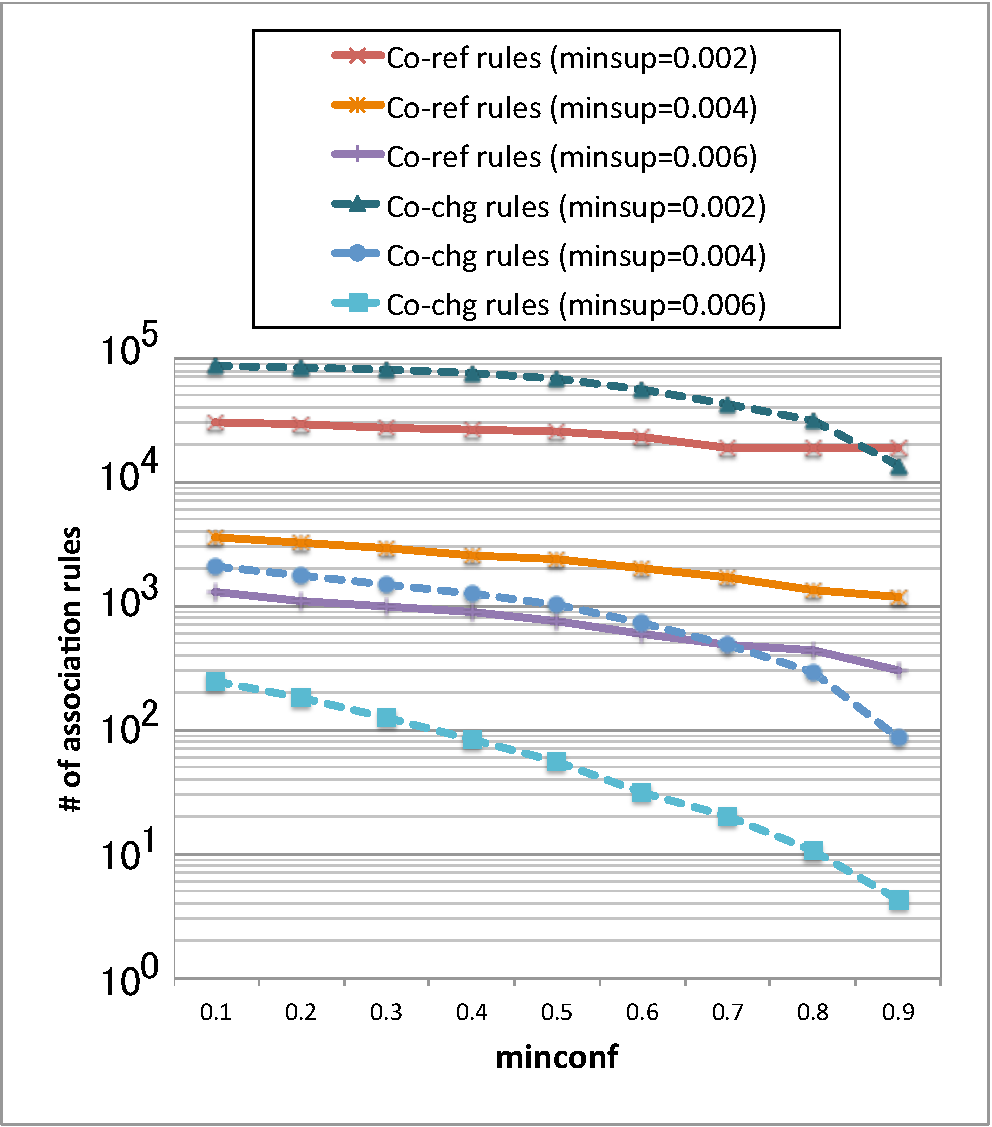
\includegraphics[width = 0.95\linewidth]{resource/rulesize_f.pdf}
  \caption{ファイルレベルでの相関ルール数}
  \label{f_rule}
\end{figure}
\begin{figure}[p]
  \centering
  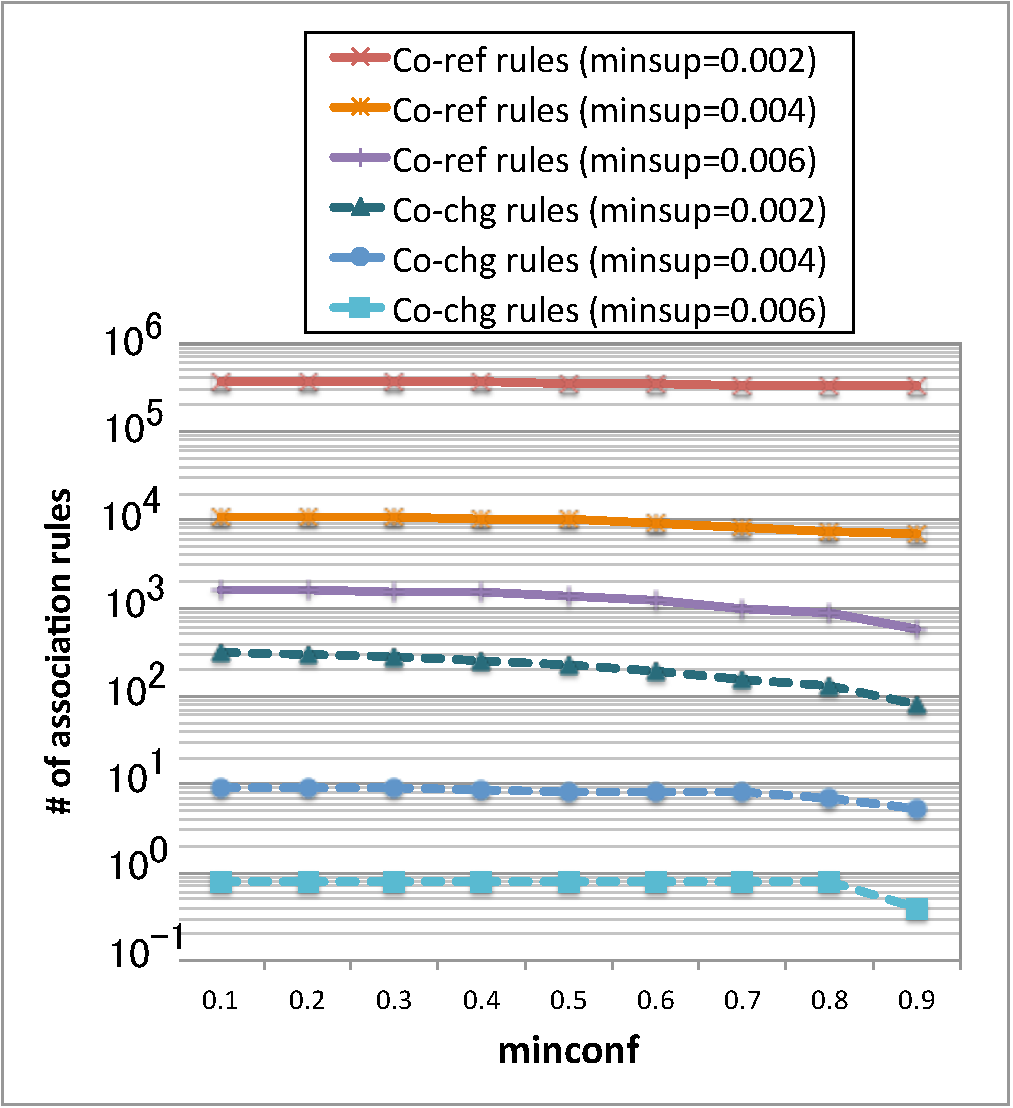
\includegraphics[width = 0.95\linewidth]{resource/rulesize_m.pdf}
  \caption{メソッドレベルでの相関ルール数}
  \label{m_rule}
\end{figure}
ファイルレベルとメソッドレベルでの抽出できた相関ルールの個数を、図\ref{f_rule}および図\ref{m_rule}にそれぞれ示す。
実線はco-refルールを、破線はco-chgルールを表す。
10-分割交差検定を行ないその平均値を表示しているため、メソッドレベルの結果の一部では、ルールの個数が1未満となるものが含まれている。

図\ref{m_rule}から、メソッドレベルにおいて、参照履歴から抽出した相関ルールが、改版履歴から抽出した相関ルールよりも多いことがわかる。
メソッドレベルのco-refルールとco-chgルールの個数の差は同一の$minsup$パラメータで比較した時1000倍以上である。
それに対し、図\ref{f_rule}のように、ファイルレベルでは参照履歴から抽出した相関ルールと改版履歴から抽出した相関ルールでメソッドレベルほどの大きな差がなかった。
ファイルレベルのco-refルールとco-chgルールの個数の差は同一の$minsup$パラメータで比較した時、最も大きいところでも10倍程度で、一部の$minsup$,$\minconf$パラメータではco-chgのほうがルールの個数が多いことがあった。

co-ref,co-chg間でのルールサイズの差がメソッドレベルとファイルレベルの相関ルールで異なった理由として、トランザクションに含まれるアイテム(成果物)の個数の特徴が異なることが考えられる。
メソッドレベルにおいては、参照セットに含まれるメソッド数の平均値は15.1個であり、変更セットの7.6個の約2倍であった。
これに対し、ファイルレベルにおいては、参照セットに含まれるメソッド数の平均値は6.5個であり、変更セットの4.9個の約1.3倍であり、ファイルレベルにおいてはメソッドレベルと比べて変更セット参照セット含まれるアイテム数の差が開いていなかった。
この事実は、開発者がメソッドを見る(カーソルをメソッドブロックの内部に入れる)とき、変更の必要のないメソッドを見ている割合がファイルを見る時と比べて多いことを示唆している。

実験対象のGitリポジトリ({\it mylyn.tasks})の調査したところ、最新コミットでは存在しないファイルやメソッドも含め、1793のJavaファイルと17040のメソッドが存在した。
ただし、この数はファイルやメソッドがリネームされた場合は1つのファイルやメソッドとして数える。
相関ルールに含まれている成果物の数に注目すると、前述のトランザクションに含まれる成果物数と同様の傾向があった。
最も多くのルールを抽出できるパラメータで相関ルールを抽出したとき、メソッドレベルにおいては、co-refルールには1112メソッドが含まれており、全体のメソッド数の6.5\%であったのに対し、co-chgルールには119メソッドが含まれており、全体のメソッド数の0.70\%しか含まれていなかった。
ファイルレベルにおいては、co-refルールとco-chgルールではほぼ同数のファイルが含まれていた。
co-refルールには、490ファイルが含まれており、全体のファイル数の27\%出会ったのに対し、co-chgルールには463ファイルが含まれており、全体のファイル数の26\%であった。

\ref{extractrules_sec}節で述べたように、参照履歴ではコミット-セッションペアが作成できたトランザクションのみを、変更履歴ではコミット-セッションペアが作成できたかどうかにかかわらず全てのトランザクションを学習セットとするため、
参照履歴の学習セットに含まれるトランザクション数は変更履歴よりも少ない。
抽出される相関ルールは$minsup$によって足切りをされるため、\ref{joining_sec}節で述べたようにすべての参照セットは変更セットを包含しているにもかかわらず、co-chgルールに含まれるルールがco-refルールに含まれない可能性がある。
実際、最も多くのco-chgルールを含んでいたco-refルールにおいてもその割合は$\frac{|\textrm{co-ref~} \cap \textrm{~co-chg}|}{|\textrm{co-chg}|}=45\%$であった。

ルール数についてまとめると、以下のことが言える。
\begin{quote}
ルールの正確さや有用性についてを無視した場合、メソッドレベルにおいては、操作履歴と改版履歴を結合した参照履歴から得られる相関ルールは改版履歴のみから得られる相関ルールよりも多くのメソッドを含めることができる。
これに対し、ファイルレベルにおいては、2種類の相関ルールはほぼ同数のファイルを含めることができる。
\end{quote}

\section{$MRR$と$Recall$、$\fmeasure$}
\begin{figure}[p]
  \centering
  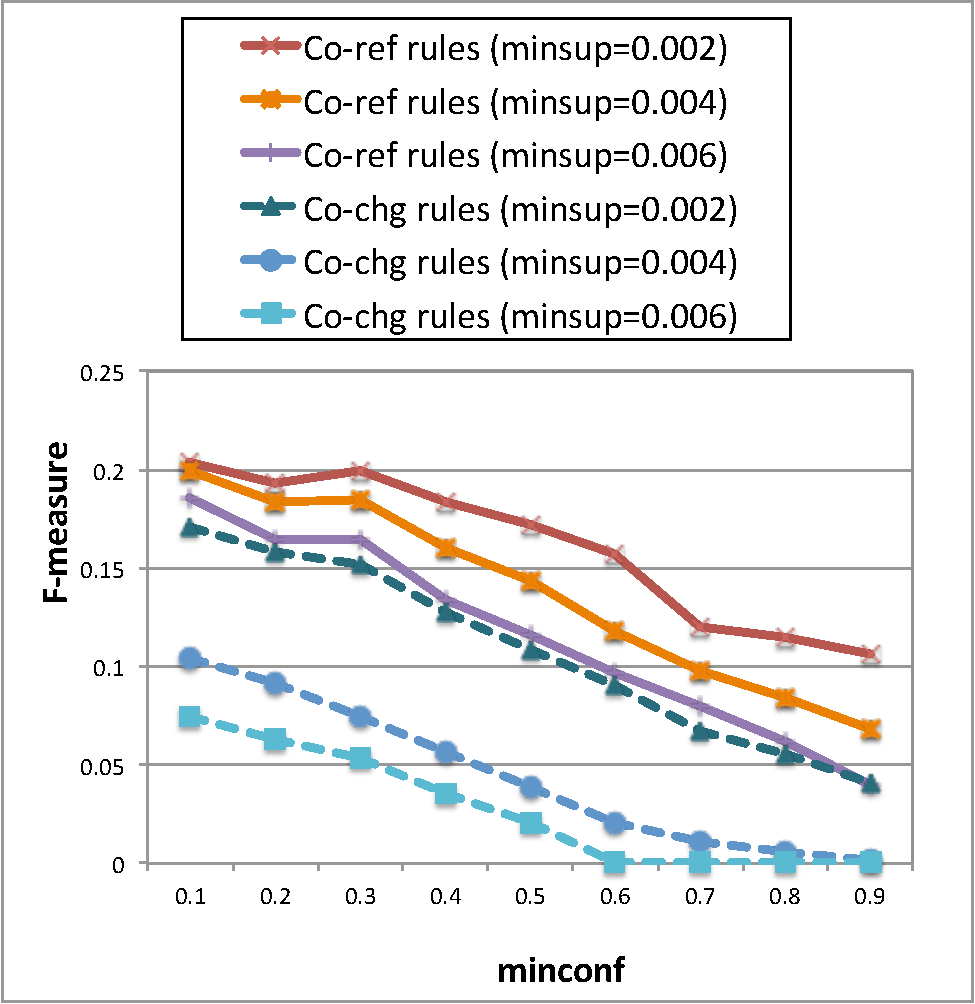
\includegraphics[width = 0.95\linewidth]{resource/fmeasure_f.pdf}
  \caption{ファイルレベルにおける$\fmeasure$}
  \label{f_fmeasure}
\end{figure}
\begin{figure}[p]
  \centering
  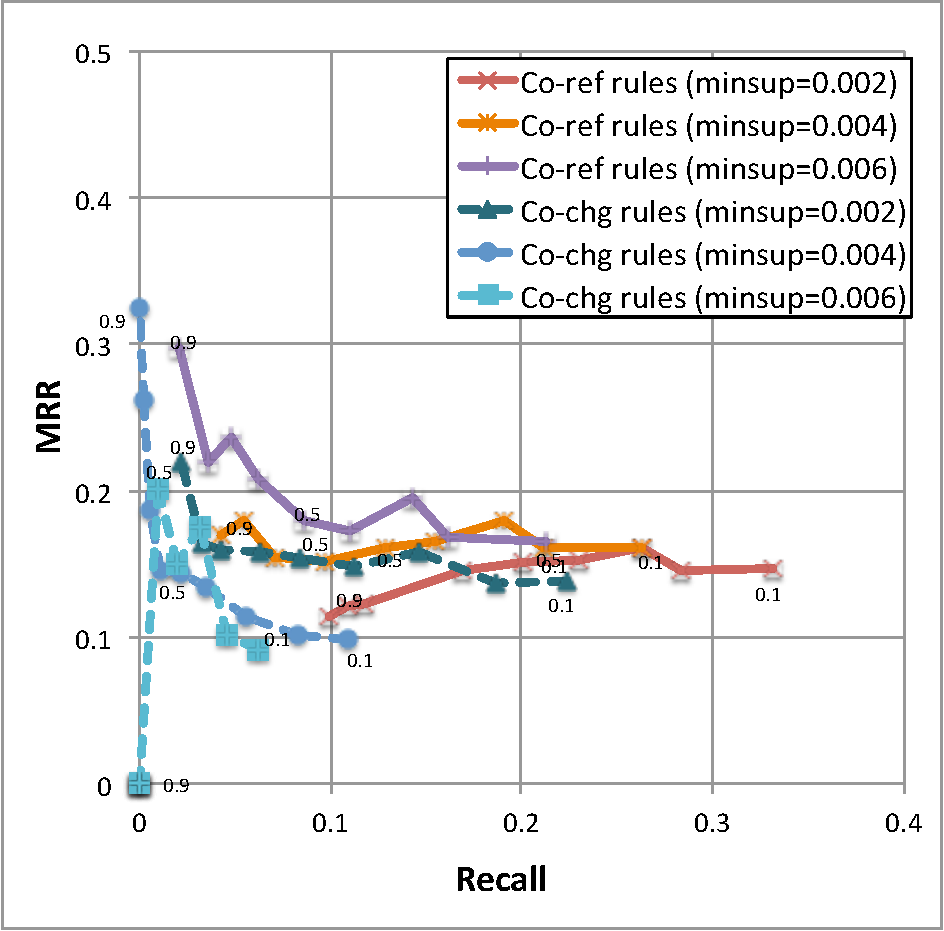
\includegraphics[width = 0.95\linewidth]{resource/mrgraph_f.pdf}
  \caption{ファイルレベルでの$MRR$と$Recall$の関係}
  \label{f_mrgraph}
\end{figure}
本節では、10-分割交差検定により実際に相関ルールを用いて変更推薦を行い、その精度を$MRR$と$Recall$およびその調和平均である$\fmeasure$から評価する。
メソッドレベルとファイルレベルにおける$\fmeasure$を、図\ref{f_fmeasure}と図\ref{m_fmeasure}に、$MRR$と$Recall$の関係を、図\ref{f_mrgraph}と図\ref{m_mrgraph}に示す。

図\ref{f_mrgraph}と図\ref{m_mrgraph}で、点に付して表示している数値は$\minconf$の値である。
メソッドレベルにおけるco-chgルールの変更推薦では、$minsup \geq 0.006$のときに変更推薦を行なうことが一切出来なかったため、$minsup = 0.006$のグラフは原点にのみプロットしている。


\subsection{ファイルレベルでの変更推薦}\label{file_result_sec}
図\ref{f_fmeasure}によれば、co-refルールを用いた時の最大$\fmeasure$は0.204 ($minsup=0.002, \minconf =0.1$)であり、co-chgルールを用いた時の最大$\fmeasure$が0.171 ($minsup=0.002, \minconf =0.1$)であったため、co-chgルールと比較してco-refルールは$\fmeasure$が19.3\%向上した。
したがって、ファイルレベルではco-refルールを使うことにより、co-chgルールを使う時と比べ変更推薦の普遍的な性能が向上したと言える。

ファイルレベルでの変更推薦で特筆すべき点として、\ref{rulesize_sec}節で見たように$minsup=0.002,\minconf \leq 0.008$のパラメータにおいて、co-refルールに含まれるルール数がco-chgルールよりも少ないのにもかかわらず、co-refルールにより$\fmeasure$が向上したことが挙げられる。
この事実は、co-refルールには、co-chgルールよりも変更推薦に有益なルールが多く含まれ、かつ変更推薦の役に立たないルールが少ないことを表しており、
参照履歴を使う変更推薦が変更履歴を使うよりも適切な変更推薦を効率的に行えることを示している。

\begin{table}[t]
  \begin{center}
    \caption{ファイルレベルの実験結果の代表値}
    \label{results_file_table}
    \begin{tabular}{l|lll|lll}
      \hline
       & \multicolumn{3}{|c|}{co-refルール} & \multicolumn{3}{|c}{co-chgルール}\\
       &$MRR$ & $Recall$ & $(minsup,\minconf)$ & $MRR$ & $Recall$ & $(minsup,\minconf)$ \\
      \hline
      最大$MRR$ &0.298&{\bf 0.021} & (0.006, 0.9) &0.325&0.0006 & (0.004, 0.9)\\
      (推薦可能な回数)            &&(12.6回) &&& (0.3回)\\
      \hline
      最大$Recall$    &0.147&{\bf 0.332} & (0.002, 0.1) &0.138&0.224 & (0.002, 0.1) \\
      \hline
      $Recall > 0.1$のときの &{\bf 0.196}& 0.143 & (0.006, 0.3) &0.158&0.146 & (0.002, 0.3) \\
      最大$MRR$&&&&&\\
      \hline
    \end{tabular}
  \end{center}
\end{table}

表\ref{results_file_table}は、図\ref{f_mrgraph}をもとに、一部の重要な結果を抜き出して表にまとめたものである。
最大の$MRR$を記録したのはco-chgルールであり、このときの$MRR$は0.325、パラメータは$minsup=0.004,\minconf=0.9$のときであった。
対してco-refルールの最大$MRR$は0.298であり($minsup=0.006,\minconf=0.9$)、co-chgルールの最大$MRR$より8.3\%低かった。
しかし、変更の必要な箇所を列挙し変更のし忘れを防ぐという点で、変更推薦においては$MRR$と同等かそれ以上に$Recall$が重要であると考えられる。
この観点から考えると、 co-chgルールが最大$MRR$を記録したパラメータでは、$Recall$は0.0006であった。
この数値は、600トランザクションを10-分割交差検定する間に変更推薦に成功した回数が1回未満であることを表し、ほとんどのコミットで変更推薦をすることが出来ないため有益な変更支援とはいえない。

一方、最大の$Recall$を記録したのはco-refルールであり、このときの$Recall$は0.332、パラメータは$minsup=0.002,\minconf=0.1$のときであった。
対してco-refの最大$Recall$は0.224であり($minsup=0.002,\minconf=0.1$)、co-refルールはco-chgルールの最大$Recall$から48\%向上した。
これは、co-refルールを用いることによって、変更し忘れる可能性のあるファイルを3ファイルのうち1ファイル見つけることができることを表している。
さらに、$Recall$が0.1以上であるときに限定すると、co-refルールによる$MRR$の最大値は0.196($minsup=0.006,\minconf=0.3$)となりco-chgルールの$MRR$の最大値0.158($minsup=0.002,\minconf=0.3$)より24\%向上している。
したがって、co-refルールを使うことでco-chgルールを使った時よりも、変更を見逃す可能性のあるファイルをより多く推薦することが可能となること、及び推薦できる回数を固定した場合には推薦の精度が向上することが示された。

\begin{table}[t]
  \begin{center}
    \caption{ウィルコクソンの符号順位検定のP値 (ファイルレベル)}
    \label{pvalue_file}
    \begin{tabular}{l|rrr}
      \hline
      $minsup$ & $\fmeasure$ & $MRR$ & $Recall$\\
      \hline
      0.002 & {\bf 0.012} & 0.975 & {\bf 0.009}\\
      0.004 & {\bf 6.2e-4} & 0.129 & {\bf 0.002}\\
      0.006 & {\bf 0.009} & 0.030 & {\bf 0.014}\\
      \hline
    \end{tabular}
  \end{center}
\end{table}

表\ref{pvalue_file}は、帰無仮説「co-refルールを用いた変更推薦の各メトリクスはco-chgルールを用いたときと比べ差がないか悪化する」を、ウィルコクソンの符号順位検定によって$minsup$毎に片側検定したものである。
ただし、co-chgルールで変更推薦した際$minsup=0.006$のパラメータにおいて$MRR=Recall=0$となる結果が存在するため、この結果は検定時に除外した。
表中で太字となっている数値は、有意水準$p=0.025$において有意差が存在した部分であり、全ての$minsup$において、co-refルールによる変更推薦の$\fmeasure$と$Recall$の分布はco-chgルールよりも大きいことが示された。

\subsection{メソッドレベルでの変更推薦}\label{method_result_sec}

\begin{figure}[p]
  \centering
  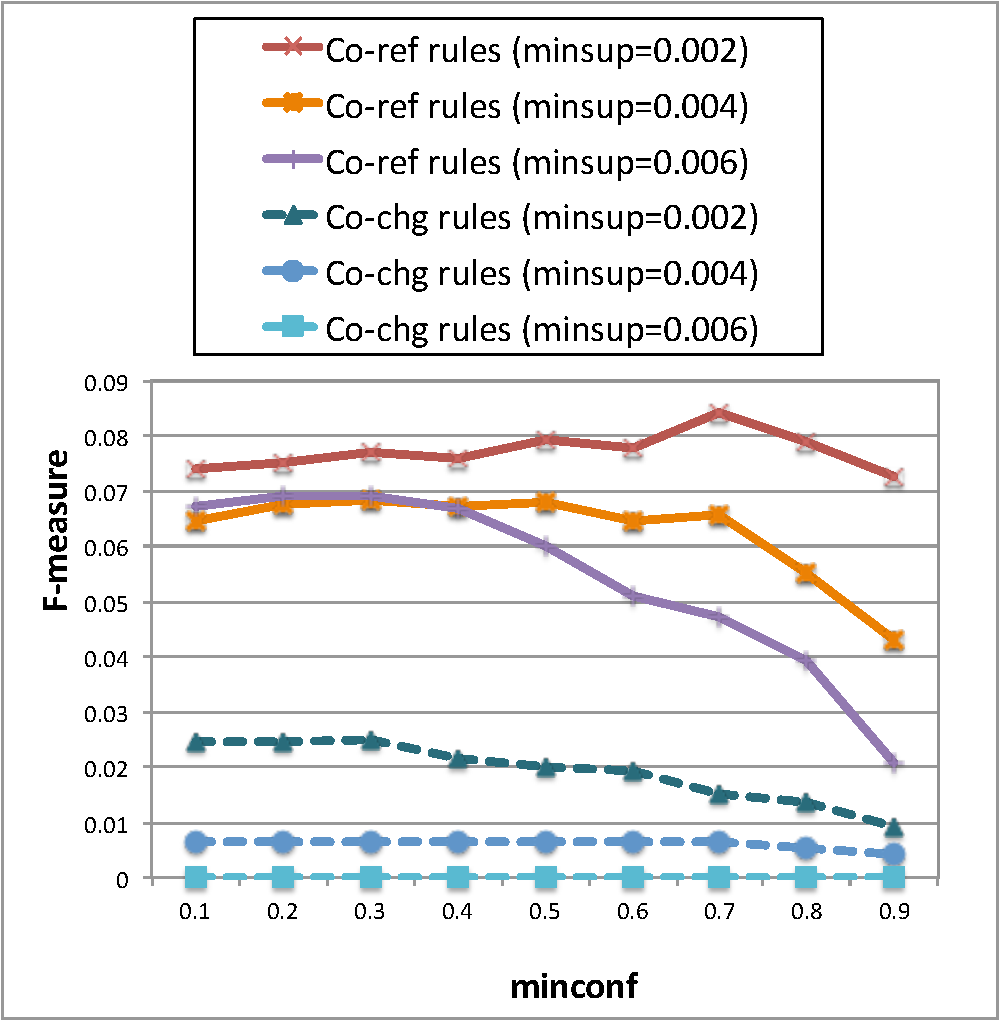
\includegraphics[width = 0.95\linewidth]{resource/fmeasure_m.pdf}
  \caption{メソッドレベルにおける$\fmeasure$}
  \label{m_fmeasure}
\end{figure}
\begin{figure}[p]
  \centering
  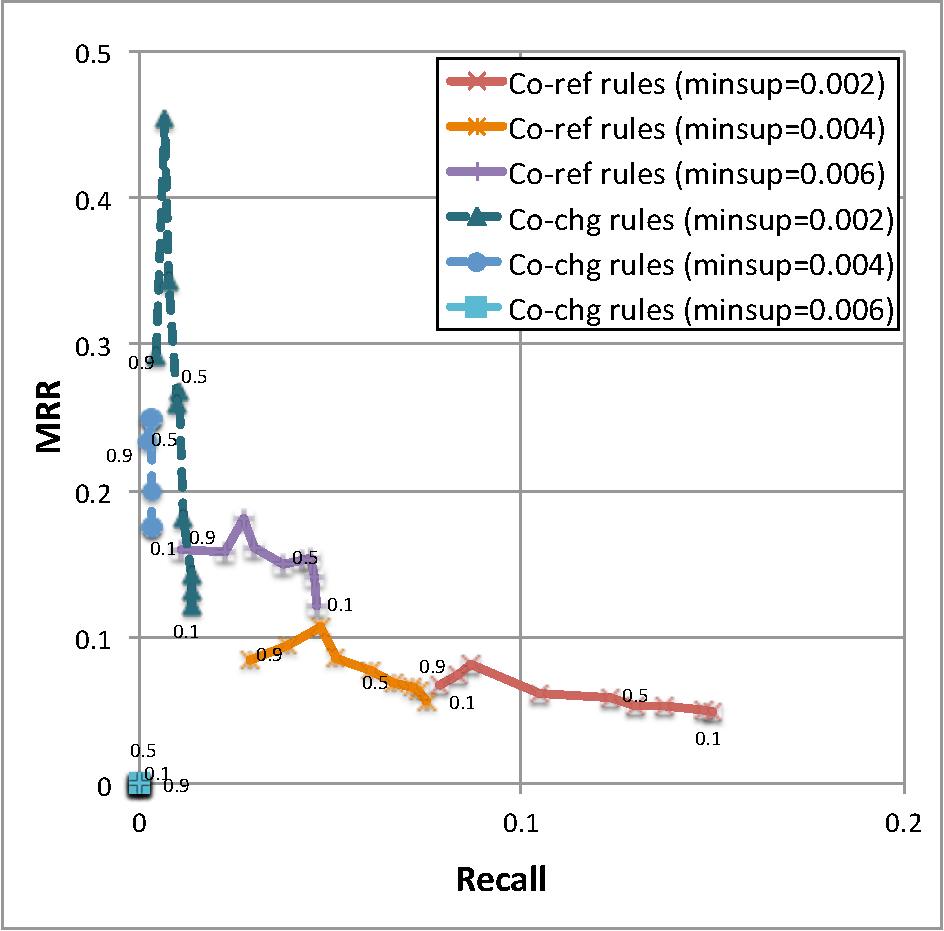
\includegraphics[width = 0.95\linewidth]{resource/mrgraph_m.pdf}
  \caption{メソッドレベルでの$MRR$と$Recall$の関係}
  \label{m_mrgraph}
\end{figure}
メソッドレベルの変更推薦の$\fmeasure$はファイルレベルの変更推薦と同様の傾向を示している(図\ref{m_fmeasure})。
メソッドレベルの変更推薦におけるco-refルールを用いた時の最大$\fmeasure$は$0.084$ ($minsup=0.002,\minconf=0.7$)であり、co-chgルールを用いた時の最大$\fmeasure$は0.025 ($minsup=0.002,\minconf=0.3$)であったため、co-chgルールと比較してco-refルールは$\fmeasure$が3.4倍となった。
しかし、メソッドレベルにおけるco-refルールの最大$\fmeasure$はファイルレベルにおけるco-refルールの最大$\fmeasure$(0.204)の41\%であり、大きく下がってしまっている。
したがって、メソッドレベルのco-refルールを使うことにより、co-chgルールを使う時と比べ変更推薦の普遍的な性能が向上したと言えるが、一方でファイルレベルのco-refルールよりは劣ることが示された。

図\ref{m_mrgraph}では、co-refルールによるメソッドレベルの最大$Recall$は0.150であり、ファイルレベルの最大$Recall$(0.332)の半分以下となっている。
メソッドレベルの変更推薦でco-refルールの$Recall$が減少した原因として、co-refルールに多くの無駄な相関ルールが含まれていることが考えられる。
例えば、開発者がある機能のメンテナンスを行なうためにその機能に関連したメソッドを変更する場合について考える。
このとき、開発者はその機能のメンテナンスを行なうために変更の必要なメソッドとそのメソッドを変更したときに変更が伝播するメソッドを探す必要があり、多くの関係のないメソッドを参照することになる。
このような開発者の行動が操作履歴に記録されていると、多くの無益なco-refルールが抽出されることとなり、適切な変更推薦を行えなくなる。
対してファイルレベルにおいては、ある機能に関連したメソッドは多くの場合同じファイル内に記述されているため、メソッドレベルのように無益なco-refルールが抽出されることは起きなかったと考えられる。

\begin{table}[t]
  \begin{center}
    \caption{ウィルコクソンの符号順位検定のP値 (メソッドレベル)}
    \label{pvalue_method}
    \begin{tabular}{l|rrr}
      \hline
      $minsup$ & $\fmeasure$ & $MRR$ & $Recall$\\
      \hline
      0.002 & {\bf 2.1e-5} & 1.000 & {\bf 2.0e-4}\\
      0.004 & {\bf 2.0e-4} & 1.000 & {\bf 1.4e-4}\\
      \hline
    \end{tabular}
  \end{center}
\end{table}

表\ref{pvalue_method}は、帰無仮説「co-refルールを用いた変更推薦の各メトリクスはco-chgルールを用いたときと比べ差がないか悪化する」を、ウィルコクソンの符号順位検定によって$minsup$毎に片側検定したものである。
ただし、$minsup=0.006$のとき、co-chgルールはすべてのパラメータで$MRR=Recall=0$だったため、表\ref{pvalue_method}に含めなかった。
表中で太字となっている数値は、有意水準$p=0.025$において有意差が存在した部分であり、全ての$minsup$において、co-refルールによる変更推薦の$\fmeasure$と$Recall$の分布はco-chgルールよりも大きいことが示された。

\subsection{ファイルレベル、メソッドレベルにおける変更推薦のまとめ}
\ref{file_result_sec}節および\ref{method_result_sec}節の結果をまとめると以下のようになる。

まず、ファイルレベルとメソッドレベルの両方において、操作履歴を用いて抽出した相関ルールは、改版履歴のみから抽出した相関ルールと比べ有意に$\fmeasure$を向上させることができたため、変更推薦の普遍的な性能が向上したと言える。
実験結果の詳細を見ると、操作履歴を用いて相関ルールを抽出することにより、変更すべき成果物の検出割合が大きく改良され、また、検出割合が同数になるようなパラメータで変更推薦を行なうと、その推薦精度が向上することがわかった。
推薦精度が最大となるようパラメータを調整すると、操作履歴から抽出した相関ルールは改版履歴から抽出した相関ルールよりも推薦精度が悪化したが、これは「変更漏れを防ぐ」という変更推薦の目的を考えると、推薦精度よりも成果物の検出割合のほうが重要であり、推薦精度の悪化は許容できる。
したがって全体としては、操作履歴を用いて変更推薦を行うことにより、改版履歴のみを用いるよりも変更推薦の効果を高めることが出来たといえる。

ファイルレベルの変更推薦では相関ルールの数が増えることなく変更推薦の性能が向上した。
これは、操作履歴を用いて相関ルールを抽出するとより多くの有益な相関ルールを抽出できると同時に有益でない相関ルールが減ったことを示しており、
このことからも操作履歴から抽出した相関ルールは有益であるといえる。

メソッドレベルの変更推薦においては、変更すべき成果物の検出割合はファイルレベルの変更推薦の半分以下となった。
これは、ファイルレベルとくらべ、開発者は機能のメンテナンスを行なう際により多くの関係のないメソッドを参照するため、このような参照行動が操作履歴に記録され、ここから有益でない相関ルールが抽出されてしまったためと考えられる。
\section{共参照ルールが有効だった変更推薦の例}
交差検定を実施した際、co-chgの相関ルールでは変更推薦の候補を出力することが出来なかったが、co-refの相関ルールでは正しく変更推薦を行えた場合があった。
このときの状況について説明する。

あるコミットには以下の4つのファイルが含まれていた。
\begin{itembox}{コミットに含まれていたファイル名}
  /tasks/ui/search/RepositorySearchResultView.java \\
  /tasks/ui/search/SearchResultContentProvider.java \\
  /tasks/ui/search/SearchResultTreeContentProvider.java \\
  /tasks/ui/TaskSearchPage.java
\end{itembox}
このコミットと結合されたセッションには、以上のファイルに加えさらに合計で7つのファイルが含まれていた。
\begin{itembox}{セッションに含まれていたファイル名}
  (コミットに含まれている4ファイル)\\
  /tasks/ui/views/TaskListContentProvider.java \\
  /tasks/ui/search/SearchResultTableContentProvider.java\\
  /tasks/ui/wizards/AbstractRepositoryQueryPage.java
\end{itembox}
ただし、これらのファイルはすべて"/org/eclipse/mylyn/internal/"フォルダの下にあり、上記のリストではこのフォルダ以下のファイルパスを記載している。

このコミットを評価する際、co-chgの相関ルールには適用可能なものがなかったのに対し、co-refの相関ルールでは以下の4つの相関ルールが適用可能であった。
\begin{itembox}{適用可能なco-refの相関ルール}
  \begin{enumerate}
    \item  \{SearchResultContentProvider.java\} $\Rightarrow$ RepositorySearchResultView.java
    \item \{SearchResultContentProvider.java\} $\Rightarrow$ SearchResultTreeContentProvider.java
    \item \{SearchResultContentProvider.java, ~SearchResultTreeContentProvider.java\} 
      \\$\Rightarrow$ RepositorySearchResultView.java
    \item \{SearchResultContentProvider.java, ~RepositorySearchResultView.java\} \\
  $\Rightarrow$ SearchResultTreeContentProvider.java
  \end{enumerate}
\end{itembox}

1番目のルール(\{SearchResultContentProvider.java\} $\Rightarrow$ RepositorySearchResultView.java)に注目する。
SearchResultContentProviderはEclipseのビューの一部分(View part)を提供する機能が実装されているクラスであり、抽象クラスである。
また、このクラスはRepositorySearchResultViewクラスにある8つのフィールド変数のうちの一つであり、
RepositorySearchResultViewを変更しようとする開発者は、一貫性が維持できているか確認するためSearchResultContentProviderを参照する必要がある。
したがって、操作履歴上には開発者がこれらのファイルを同時に参照したことが何度も記録され、その結果操作履歴を用いて"\{SearchResultContentProvider.java\} $\Rightarrow$ RepositorySearchResultView.java"の相関ルールが抽出され、このコミットで正しく変更推薦を行なうことが出来た。

しかし、この2つのファイル間に張られるようなco-chgの相関ルールは抽出されなかった。
これはSearchResultContentProviderが改版履歴上で変更されることがほとんどなかったためである。

この例のように、変更されることが少ないファイルに対する相関ルールを抽出することができ、そのような相関ルールで実際に正しい変更推薦を行える点で、操作履歴を用いた変更推薦は改版履歴のみを用いるより推薦精度が向上したと考えられる。

\section{妥当性への脅威}
\subsection{内的妥当性}
本研究ではBugzillaウェブサイトをクローリングすることでMylynログを収集した。
BugzillaにアップロードされているMylynログはプログラムの編集時に開発者の操作を記録したものだけでなく、Mylynプラグインの利用者がクラッシュリポートとしてアップロードしたものも含まれている。
しかし、これらを区別する方法がないため、開発者の操作が記録されたMylynログとクラッシュリポートのMylynログを区別せずに用いている。
Gitの改版履歴と結合する際に、作成日時の差を2分以内とするなど厳しい条件を使っているためほとんどのクラッシュリポートのMylynログは除去されているものと考えられるが、偶然条件が揃った場合はクラッシュリポートのMylynログを結合している可能性がある。
\TODO{}
\subsection{外的妥当性}
\subsection{構造的妥当性}

\chapter{結論}
\TODO{}
\chapter*{謝辞}
研究を進めるにあたり、終始熱心なご指導を頂いた小林隆志先生に感謝の意を表します。

佐伯研究室の林晋平先生には、研究方針や論文の表現方法などに対し多くの助言を頂き、心より感謝しております。

奈良先端科学技術大学院大学の藤原賢二さんからは研究上必要なデータの提供の他、データの処理方法に関して助言を頂きました。ありがとうございました。

東京工業大学小林研究室の学生の皆様、同研究室の留学生の皆様、スウェーデン王立工科大学のAnders Hagwardさんには、研究への助言及び実験補助、自作ライブラリやツールの提供等、研究上不可欠な援助を頂きましたことを深く感謝いたします。

小林研究室秘書の高野さん、三寺さんには、研究上必要な事務処理をしていただいた他、研究上思い悩む点について相談させていただいたことなど、研究遂行のための支えとなりました。
ありがとうございました。

\appendix
\chapter{拡張したMylynによって取得できる操作履歴ログファイルの例}\label{mylyn_log_appendix}
\lstinputlisting[language=xml]{local-2.xml}
\chapter{Mylynプロジェクトに含まれるGitリポジトリの一覧}\label{mylyn_repo_appendix}
\begin{itemize}
\item {\it mylyn.builds} (\url{https://github.com/eclipse/mylyn.builds})
\item {\it mylyn.docs.vex} (\url{https://github.com/eclipse/mylyn.docs.vex})
\item {\it mylyn.tasks} (\url{https://github.com/eclipse/mylyn.tasks})
\item {\it mylyn.reviews} (\url{https://github.com/eclipse/mylyn.reviews})
\item {\it mylyn.versions} (\url{https://github.com/eclipse/mylyn.versions})
\item {\it mylyn.incubator} (\url{https://github.com/eclipse/mylyn.incubator})
\item {\it mylyn.context} (\url{https://github.com/eclipse/mylyn.context})
\item {\it mylyn.docs} (\url{https://github.com/eclipse/mylyn.docs})
\item {\it mylyn.commons} (\url{https://github.com/eclipse/mylyn.commons})
\item {\it mylyn.docs.intent.main} (\url{https://github.com/eclipse/mylyn.docs.intent.main})
\item {\it mylyn.reviews.r4e} (\url{https://github.com/eclipse/mylyn.reviews.r4e})
\item {\it mylyn} (\url{https://github.com/eclipse/mylyn})
\end{itemize}


\backmatter
\bibliographystyle{junsrt}
\bibliography{bibtex/citation}
% 最終稿段階で .bbl に細かい修正を入れること.

\end{document}
